\documentclass[11pt,twoside, french]{StyleThese}



%\input{structure}

\include{formatAndDefs}




%%% TEMPLATE POUR PARTIE EN BLEU
\iffalse
\usepackage{fourier}% change to lmodern if fourier is no available
\usepackage{tikz}
\usepackage[explicit]{titlesec}

\definecolor{mybluei}{RGB}{0,173,239}
\definecolor{myblueii}{RGB}{63,200,244}
\definecolor{myblueiii}{RGB}{199,234,253}

\renewcommand\thepart{\arabic{part}}

\newcommand\partnumfont{% font specification for the number
  \fontsize{380}{130}\color{myblueii}\selectfont%
}

\newcommand\partnamefont{% font specification for the name "PART"
  \normalfont\color{white}\scshape\small\bfseries 
}

\titleformat{\part}
  {\normalfont\huge\filleft}
  {}
  {20pt}
  {\begin{tikzpicture}[remember picture,overlay]
  \fill[myblueiii] 
    (current page.north west) rectangle ([yshift=-13cm]current page.north east);   
  \node[
      fill=mybluei,
      text width=2\paperwidth,
      rounded corners=6cm,
      text depth=18cm,
      anchor=center,
      inner sep=0pt] at (current page.north east) (parttop)
    {\thepart};%
  \node[
      anchor=south east,
      inner sep=0pt,
      outer sep=0pt] (partnum) at ([xshift=-20pt]parttop.south) 
    {\partnumfont\thepart};
  \node[
      anchor=south,
      inner sep=0pt] (partname) at ([yshift=2pt]partnum.south)   
  {\partnamefont PART};
  \node[
      anchor=north east,
      align=right,
      inner xsep=0pt] at ([yshift=-0.5cm]partname.east|-partnum.south) 
  {\parbox{.7\textwidth}{\raggedleft#1}};
  \end{tikzpicture}%
  }
  \fi

%WORK
\iffalse
% standard incantations
\usepackage[T1]{fontenc}
\usepackage[utf8]{inputenc}
\usepackage{lmodern}
% glossary
\usepackage[xindy]{glossaries} 
\usepackage[index]{glossaries}
\newglossaryentry{domain-knowledge}{%
  name={domain knowledge},%
  description={valid knowledge used to refer to an area of human endeavour, an autonomous computer activity, or other specialized discipline}}

\newacronym{tla}{TLA}{Three Letter Acronym}




\newglossaryentry{latex}
{
    name=latex,
    description={Is a mark up language specially suited for scientific documents}
}

\newglossaryentry{maths}
{
    name=mathematics,
    description={Mathematics is what mathematicians do}
}

\newglossaryentry{formula}
{
    name=formula,
    description={A mathematical expression}
}



\newglossaryentry{duck}{name=DUUuck,
  description={a waterbird with webbed feet}}

\newglossaryentry{parrot}{name=Parrot,
  description={mainly tropical bird with bright plumage}}
  
  %%% The glossary entry the acronym links to   
\newglossaryentry{apig}{name={API},
    description={An Application Programming Interface (API) is a particular set
of rules and specifications that a software program can follow to access and
make use of the services and resources provided by another particular software
program that implements that API}}

%%% define the acronym and use the see= option
\newglossaryentry{api}{type=\acronymtype, name={API}, description={Application
Programming Interface}, first={Application
Programming Interface (API)\glsadd{apig}}}



  %%% The glossary entry the acronym links to   
\newglossaryentry{hpcg}{name={HPC},
    description={Le but du HPC est de paralléliser des applications scientifiques à destination de ressources informatiques telles que les supercalculateurs}}

%%% define the acronym and use the see= option
\newglossaryentry{hpc}{type=\acronymtype, name={HPC}, description={High Performance Computing ou Calcul Haute Performance}, first={Calcul Haute Performance (HPC)\glsadd{hpcg}}}




%\newglossaryentry{hpc}{%
%  name={Calcul Haute Performance},%
%  description={Le but du HPC est de paralléliser des applications scientifiques à destination de ressources informatiques telles que %les supercalculateurs}
%}


%\newabbreviation[category=common]{debs}{DEBS}{Distributed Event-Based System}

%\newabbreviation[category=common]{p2p}{P2P}{Peer-to-Peer}

%\newabbreviation[category=common]{http}{HTTP}{Hypertext Transfer Protocol}
\makeglossaries
\fi

%WORK 2
\iffalse
\usepackage{imakeidx}
\usepackage{hyperref}
\usepackage[abbreviations, xindy,acronym]{glossaries-extra}
\makeglossaries
\newglossaryentry{domain-knowledge}{%
  name={domain knowledge},%
  description={valid knowledge used to refer to an area of human endeavour, an autonomous computer activity, or other specialized discipline}}

\newacronym{tla}{TLA}{Three Letter Acronym}




\newglossaryentry{latex}
{
    name=latex,
    description={Is a mark up language specially suited for scientific documents}
}

\newglossaryentry{maths}
{
    name=mathematics,
    description={Mathematics is what mathematicians do}
}

\newglossaryentry{formula}
{
    name=formula,
    description={A mathematical expression}
}



\newglossaryentry{duck}{name=DUUuck,
  description={a waterbird with webbed feet}}

\newglossaryentry{parrot}{name=Parrot,
  description={mainly tropical bird with bright plumage}}
  
  %%% The glossary entry the acronym links to   
\newglossaryentry{apig}{name={API},
    description={An Application Programming Interface (API) is a particular set
of rules and specifications that a software program can follow to access and
make use of the services and resources provided by another particular software
program that implements that API}}

%%% define the acronym and use the see= option
\newglossaryentry{api}{type=\acronymtype, name={API}, description={Application
Programming Interface}, first={Application
Programming Interface (API)\glsadd{apig}}}



  %%% The glossary entry the acronym links to   
\newglossaryentry{hpcg}{name={HPC},
    description={Le but du HPC est de paralléliser des applications scientifiques à destination de ressources informatiques telles que les supercalculateurs}}

%%% define the acronym and use the see= option
\newglossaryentry{hpc}{type=\acronymtype, name={HPC}, description={High Performance Computing ou Calcul Haute Performance}, first={Calcul Haute Performance (HPC)\glsadd{hpcg}}}




%\newglossaryentry{hpc}{%
%  name={Calcul Haute Performance},%
%  description={Le but du HPC est de paralléliser des applications scientifiques à destination de ressources informatiques telles que %les supercalculateurs}
%}


%\newabbreviation[category=common]{debs}{DEBS}{Distributed Event-Based System}

%\newabbreviation[category=common]{p2p}{P2P}{Peer-to-Peer}

%\newabbreviation[category=common]{http}{HTTP}{Hypertext Transfer Protocol}
\input{acronymes}
\glssetcategoryattribute{common}{dualindex}{true}
\setabbreviationstyle[common]{long-short-desc}
\makeglossaries
\makeindex
\fi


\usepackage{hyperref}  %pour autoref

%%%%% GLOSSAIRE %%%%%%%
\usepackage[acronym]{glossaries}
\makeglossaries
\newglossaryentry{domain-knowledge}{%
  name={domain knowledge},%
  description={valid knowledge used to refer to an area of human endeavour, an autonomous computer activity, or other specialized discipline}}

\newacronym{tla}{TLA}{Three Letter Acronym}




\newglossaryentry{latex}
{
    name=latex,
    description={Is a mark up language specially suited for scientific documents}
}

\newglossaryentry{maths}
{
    name=mathematics,
    description={Mathematics is what mathematicians do}
}

\newglossaryentry{formula}
{
    name=formula,
    description={A mathematical expression}
}



\newglossaryentry{duck}{name=DUUuck,
  description={a waterbird with webbed feet}}

\newglossaryentry{parrot}{name=Parrot,
  description={mainly tropical bird with bright plumage}}
  
  %%% The glossary entry the acronym links to   
\newglossaryentry{apig}{name={API},
    description={An Application Programming Interface (API) is a particular set
of rules and specifications that a software program can follow to access and
make use of the services and resources provided by another particular software
program that implements that API}}

%%% define the acronym and use the see= option
\newglossaryentry{api}{type=\acronymtype, name={API}, description={Application
Programming Interface}, first={Application
Programming Interface (API)\glsadd{apig}}}



  %%% The glossary entry the acronym links to   
\newglossaryentry{hpcg}{name={HPC},
    description={Le but du HPC est de paralléliser des applications scientifiques à destination de ressources informatiques telles que les supercalculateurs}}

%%% define the acronym and use the see= option
\newglossaryentry{hpc}{type=\acronymtype, name={HPC}, description={High Performance Computing ou Calcul Haute Performance}, first={Calcul Haute Performance (HPC)\glsadd{hpcg}}}




%\newglossaryentry{hpc}{%
%  name={Calcul Haute Performance},%
%  description={Le but du HPC est de paralléliser des applications scientifiques à destination de ressources informatiques telles que %les supercalculateurs}
%}


%\newabbreviation[category=common]{debs}{DEBS}{Distributed Event-Based System}

%\newabbreviation[category=common]{p2p}{P2P}{Peer-to-Peer}

%\newabbreviation[category=common]{http}{HTTP}{Hypertext Transfer Protocol}
\input{acronymes}

%%%%% INDEX %%%%%%%%%%%
\usepackage{imakeidx}%Index compris par overleaf
\makeindex


%A chaque lien d'un mot avec sa référence dans le glosssaire
%On veut aussi mettre à jour l'index
%\iffalse
 \let\oldGls\gls
 \renewcommand{\gls}[1]{%
    \ifglsused{#1}{ %
        \oldGls{#1}%
    }{%
        \oldGls{#1}%
        \index{\glsentryfirst{#1}}%
    }%
 }
%\fi


\usepackage[many]{tcolorbox}

\usepackage{tikz}
\usetikzlibrary{arrows,automata}

\setcounter{tocdepth}{4}
\setcounter{secnumdepth}{4}

\usepackage{subcaption} %subfigure


\newcommand{\CD}[1]{\emph{\color{red} #1}}





\addto\extrasfrench{%
  \renewcommand{\equationautorefname}{équation} %Pour avoir une lettre minuscule a Équation
  \renewcommand{\lstlistingautorefname}{extrait} %Pour les extrait de code
  \renewcommand{\lstlistingname}{Extrait} %Pour les extrait de code dans la figure
}


\usepackage{listings} %citer du code

\lstset{
    escapeinside={(*}{*)}
} %pour mettre en gras un ligne (*\bfseries coucou *)




%%%%%%%%%% MATH%%%%%%%%%%%%%%%%%%%
\usepackage{empheq} %eq centrée



%%%%%%%%%%%%%%%%%%%%% POUR LE CODE %%%%%%%%%%%
\usepackage{listings}
\usepackage{color}
\usepackage{float}

%New colors defined below
\definecolor{codegreen}{rgb}{0,0.6,0}
\definecolor{codegray}{rgb}{0.5,0.5,0.5}
\definecolor{codepurple}{rgb}{0.58,0,0.82}
\definecolor{backcolour}{rgb}{0.95,0.95,0.95}

%Code listing style named "mystyle"
\lstdefinestyle{mystyle}{
  backgroundcolor=\color{backcolour},   commentstyle=\color{codegreen},
  keywordstyle=\color{blue},
  numberstyle=\tiny\color{codegray},
  stringstyle=\color{codepurple},
  basicstyle=\footnotesize,
  breakatwhitespace=false,         
  breaklines=true,                 
  captionpos=b,                    
  keepspaces=true,                 
  numbers=left,                    
  numbersep=5pt,                  
  showspaces=false,                
  showstringspaces=false,
  showtabs=false,                  
  tabsize=2
}

%"mystyle" code listing set
\lstset{style=mystyle}

%%%%%%%%%%%%%%%%%%%%%%%%%%%%%%%%%%%%%%%%%%%%%%%%%%%%%%%





\newtcolorbox{fancyquotes}{%
    enhanced jigsaw, 
    breakable,      % allow page breaks
    frame hidden,   % hide the default frame
    left=0cm,       % left margin
    right=0cm,      % right margin
    overlay={%
        \node [scale=8,
            text=black,
            inner sep=0pt,] at ([xshift=-1cm,yshift=-1cm]frame.north west){``}; 
        \node [scale=8,
            text=black,
            inner sep=0pt,] at ([xshift=1cm]frame.south east){''};  
            },
        % paragraph skips obeyed within tcolorbox
                parbox=false,
}


\begin{document}




\iffalse
The glossaries package automatically generates a list of glossary entries. It's great for keeping track of your \gls{domain-knowledge} and \glspl{tla}. In this example we've put the glossary definitions in a separate \texttt{glossary.tex} file, which you can edit via the project menu.
\\
First use \gls{debs} and \gls{p2p}. Next use: \gls{debs} and
\gls{p2p}.

No expansion: \gls{http}.
A \gls{duck} and a \gls{parrot}. Lots of \glspl{duck}.

Index aardvark\index{aardvark}.
\\
Petit test de \gls{api} et re de \gls{api}

\fi




\begin{titlepage}
\begin{center}
\noindent {\large \textbf{UNIVERSITÉ DE PARIS-SACLAY}} \\
\vspace*{0.3cm}
\noindent {\LARGE \textbf{ÉCOLE DOCTORALE DE HADAMARD}} \\
\noindent \textbf{École doctorale 574 -  Spécialité Calcul Haute Performance} \\
\vspace*{0.5cm}
\noindent \Huge \textbf{T H È S E} \\
\vspace*{0.3cm}
\noindent \large {pour obtenir le titre de} \\
\vspace*{0.3cm}
\noindent \LARGE \textbf{Docteur en Sciences} \\
\vspace*{0.3cm}
\noindent \Large de l'Université de Paris-Saclay \\
\noindent \Large \textbf{Mention : \textsc{Informatique}}\\
\vspace*{0.4cm}
\noindent \large {Présentée et soutenue par\\}
\noindent \LARGE Jean \textsc{Pourroy} \\
\vspace*{0.8cm}
\noindent {\Huge \textbf{TITRE DE LA THESE}} \\
\vspace*{0.8cm}
\noindent \Large Thèse dirigée par Christophe \textsc{Denis} et Patrick \textsc{Demichel} \\
\vspace*{0.2cm}
\noindent \Large en collaboration avec Hewlett Packard Enterprise \\
\vspace*{0.2cm}
\noindent \large soutenue le DATE \\
\vspace*{0.5cm}
\end{center}
\noindent \large \textbf{Jury :} \textbf{A FAIRE} \\
\begin{center}
\noindent \large 
\begin{tabular}{llcl}
      \textit{Rapporteurs :}	& Patrick \textsc{Clarysse}		& - & CNRS (CREATIS)\\
				& Louis \textsc{Collins}		& - & McGill University\\
      \textit{Directeur :}	& Grégoire \textsc{Malandain}		& - & INRIA (Asclepios)\\
      \textit{Président :}	& Nicholas \textsc{Ayache}		& - & INRIA (Asclepios)\\
      \textit{Examinateurs :}   & Pierre-Yves \textsc{Bondiau}          & - & Centre Antoine Lacassagne (Nice)\\
      				& Guido \textsc{Gerig}			& - & University of North Carolina\\
      				& Vincent \textsc{Grégoire}		& - & Université Catholique de Louvain\\
      \textit{Invité :}		& Hanna \textsc{Kafrouni}		& - & DOSISoft S.A.
\end{tabular}
\end{center}
\end{titlepage}
\sloppy

\titlepage


\dominitoc
\pagenumbering{roman}
\cleardoublepage



% .______       _______     _______. __    __  .___  ___.  _______  %
% |   _  \     |   ____|   /       ||  |  |  | |   \/   | |   ____| %
% |  |_)  |    |  |__     |   (----`|  |  |  | |  \  /  | |  |__    %
% |      /     |   __|     \   \    |  |  |  | |  |\/|  | |   __|   %
% |  |\  \----.|  |____.----)   |   |  `--'  | |  |  |  | |  |____  %
% | _| `._____||_______|_______/     \______/  |__|  |__| |_______| %

\section*{Résumé}
Résumé de la thèse en français

- 250 mots
- Mots clefs

\clearpage
\section*{Abstract}
Résumé de la thèse en anglais

- 250 mots
- Mots clefs


%.___  ___.  _______ .______        ______  __  
%|   \/   | |   ____||   _  \      /      ||  | %
%|  \  /  | |  |__   |  |_)  |    |  ,----'|  | %
%|  |\/|  | |   __|  |      /     |  |     |  | %
%|  |  |  | |  |____ |  |\  \----.|  `----.|  | %
%|__|  |__| |_______|| _| `._____| \______||__| %


\section*{Remerciements}

A faire en dernier :-)

\clearpage



% .___________.  ______     ______  %
% |           | /  __  \   /      | %
% `---|  |----`|  |  |  | |  ,----' %
%     |  |     |  |  |  | |  |      %
%     |  |     |  `--'  | |  `----. %
%     |__|      \______/   \______| %

\tableofcontents


%   _______  __        ______        _______.     _______.  % 
%  /  _____||  |      /  __  \      /       |    /       |  % 
% |  |  __  |  |     |  |  |  |    |   (----`   |   (----`  % 
% |  | |_ | |  |     |  |  |  |     \   \        \   \      % 
% |  |__| | |  `----.|  `--'  | .----)   |   .----)   |     % 
%  \______| |_______| \______/  |_______/    |_______/      % 
\printglossary[type=main]           % Glossaire
\printglossary[type=\acronymtype]   % Acronymes



%  ______  __    __       ___      .______   .___________. _______ .______       % 
% /      ||  |  |  |     /   \     |   _  \  |           ||   ____||   _  \      % 
%   ,----'|  |__|  |    /  ^  \    |  |_)  | `---|  |----`|  |__   |  |_)  |     % 
%   |     |   __   |   /  /_\  \   |   ___/      |  |     |   __|  |      /      % 
%   `----.|  |  |  |  /  _____  \  |  |          |  |     |  |____ |  |\  \----. % 
% \______||__|  |__| /__/     \__\ | _|          |__|     |_______|| _| `._____| % 

\mainmatter

%% PART 1 %%
\part{Introduction au contexte du Calcul Haute Performance}
%\chapter{Introduction}
\label{chap:intro}
\minitoc


 \section{Le domaine du Calcul Haute Performance} 
 

%---------------------------------------------------------------------------------

Le domaine du \gls{hpc} n'est pas apparu de lui même, c'est un moyen qui à été crée par les scientifiques et plus particulièrement ceux travaillant dans la simulation numérique. La simulation numérique est le procédé qui permet de simuler un phénomène physique sur un ordinateur par la programmation. Elle a de nombreux avantages comme celui de pouvoir simuler des phénomènes dont les conditions ne sont pas reproductibles sur terre comme dans le  domaine de la physique appliquée. Elle élargie donc les domaines explorables ce qui rend son champs d'application presque infini.  


 \subsection{Le calcul scientifique et la simulation numérique}


Les simulations sont aujourd'hui un pilier stratégique de nombreuses entreprises qui travaillent dans des domaines très différents. Pour mieux comprendre les changements qu'elle a apportée à l'industrie prenons l'exemple de l'industrie automobile et du crash de voiture. Les tests de crash de voitures ne sont plus réalisés avec de vraies voitures, les voitures sont simulées sur ordinateurs et envoyées percuter des murs virtuels. Cette technique à un impact conséquent sur le travail des ingénieurs. Elle a pour effet de réduire les temps de conception, car il n'y plus besoin de créer une voiture avec les matériaux à tester. On peut dans la même journée créer un modèle avec un matériau, lancer la simulation le temps du repas, analyser les résultats et relancer une simulation dans la nuit. Le gain de temps est énorme comparé à si on devait construire la voiture de toute pièce pour ensuite la tester sur un vrai mur. Le second gain, qui est fortement lié au premier, est la réduction des coûts de conceptions, plus besoin de faire construire des nouveaux matériaux pour se rendre compte au bout d'un essai qu'ils ne correspondent pas au besoin du constructeur. 



 
Les domaines qui ont recours au \gls{hpc} sont nombreux notamment à travers la simulation numérique qui devient un levier d'action essentiel pour beaucoup d'industries. Pour la compétitivité et l'innovation des entreprises, les simulations numériques sont désormais un outil indispensable d'aide à la conception, à la décision et au contrôle de leurs activités. Le schéma \ref{fig:tikz_simulation} montre comment la simulation numérique est venue révolutionner de nombreux domaines scientifiques.


%TikZ picture
\begin{figure}
\begin{center}

\begin{minipage}[]{.5\textwidth}

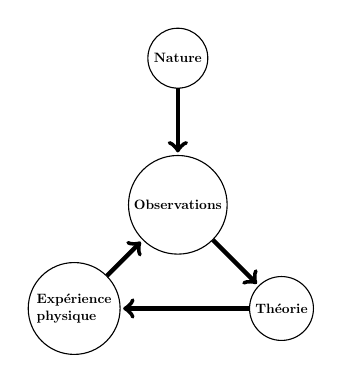
\begin{tikzpicture}[->,shorten >=1pt,auto,node distance=3.8cm,   scale=0.49, every node/.style={transform shape}]
  \tikzstyle{every state}=[fill=none,draw=black,text=black,  , font=\bf]
  \tikzstyle{edge_style} = [draw=black, line width=2, ultra thick]
  \tikzstyle{node_style} = [circle,draw=blue,fill=blue!20!,font=\sffamily\Large\bfseries]


  \node[state]					    (A)                     {Nature};
  \node[state]        				(B) [below of=A]        {Observations};
  \node[state,]         		    (D) [below right of=B]  {Théorie};
  \node[state, align=left]         	(C) [below left of=B]   {Expérience\\ physique};

  \path
		(A) edge [edge_style]   node {} (B)
        (B) edge [edge_style]   node {} (D)
        (C) edge [edge_style]   node {} (B)
        (D) edge [edge_style]   node {} (C);
\end{tikzpicture}
\end{minipage}%
\begin{minipage}[]{.5\textwidth}

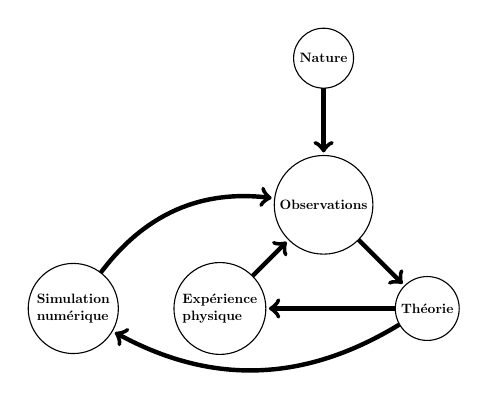
\begin{tikzpicture}[->,shorten >=1pt,auto,node distance=3.8cm,   scale=0.49, every node/.style={transform shape}]
  \tikzstyle{every state}=[fill=none,draw=black,text=black,  , font=\bf]
\tikzstyle{edge_style} = [draw=black, line width=2, ultra thick]
\tikzstyle{node_style} = [circle,draw=blue,fill=blue!20!,font=\sffamily\Large\bfseries]


  \node[state]					(A)                    {Nature};
  \node[state]        					(B) [below of=A] {Observations};
  \node[state,]         					(D) [below right of=B] {Théorie};
  \node[state, align=left]         	(C) [below left of=B] {Expérience\\ physique};
  \node[state, align=left]        	(E) [left of=C]       {Simulation\\numérique};

  \path
		(A) edge [edge_style]            node {} (B)
        (B) edge [edge_style]     node {} (D)
        (C) edge [edge_style]           node {} (B)
        (D) edge [edge_style]             node {} (C)
              edge [edge_style, bend left]     node {} (E)
        (E) edge [edge_style, bend left]  node {} (B);
\end{tikzpicture}


\end{minipage}
\end{center}


 \caption{La simulation numérique a apportée une nouvelle façon d'expérimenter les théories \cite{BSC_FIB_SCA}} 
 \label{fig:tikz_simulation}
 \end{figure}

A l'origine, les scientifiques observaient la nature et émettaient des théories pour expliquer ces observations. En se basant sur ces théories ils réalisaient des expériences physiques pour les valider ou non. Il faisaient alors de nouvelles observations pour affiner leur théorie. Les simulations numériques sont alors apparues comme des alternatives aux expériences physiques qui étaient souvent longues et onéreuses. Avec l'apparition d'ordinateurs de plus en plus puissant on pouvait donc les programmer pour simuler des expériences sans avoir à les réaliser. Les gains de temps et d'argent étant alors conséquents.

La simulation numérique est un domaine ou les programmes sont utilisés pour simuler un phénomène réel (physique, chimique, biologique, etc.). Cette approche est largement utilisée en science pour prédire l'évolution d'un phénomène dans le temps et l'espace. La majorité de ces simulations son basés sur des équations dites \textit{gouvernantes} qui sont des approximations des phénomènes étudiés. Comme les ordinateurs ne peuvent pas exécuter une infinité d'instructions, ces équations ne peuvent pas être utilisées directement et ont besoin d'être discrétisé. En mathématiques, la discrétisassions est un procédé  qui permet de passer d'une fonction, d'un modèle ou d'une équation continue à son équivalent continu (\autoref{pic_maillage}). Ce procédé ne permet pas de décrire le phénomène réel, mais de l'approximer avec plus ou moins d'erreur. Pour améliorer ces simulations, ces représentations doivent utiliser des maillages le plus fin possible. C'est en cela que ces simulations nécessitent d'énormes puissances de calculs et que cette demande est illimité car les maillages pourront toujours être affinés. 

\begin{figure}
    \center
    \includegraphics[width=4cm]{images/Chapitre1/maillage.png}
    \caption{\label{pic_maillage} Le maillage le plus fin exploité par Météo-France pour ses prévisions régionales restitue des mailles de 2,5 km de côté. (source \url{www.irma-grenoble.com})}
\end{figure}




\begin{enumerate}
\item Aéronautique: la Dynamique des Fluides (CFD) est utilisée pour valider qu'un flux d'air circule correctement autour des ailes pour essayer de maximiser le portage des ailes. 
\item Industries des hydrocarbures: la recherche pétrolière utilise le HPC pour analyser les fonds marins et modéliser les réservoirs de pétrole pour optimiser leur extraction.
\item Météorologie: pour améliorer les prédictions météorologiques mais aussi de les réaliser plus longtemps à l'avance. 
\item Sciences biologique: séquençage et alignement ADN, découverte de drogues 
\end{enumerate}



%%%%%%%%%%%%%%%%%%%%%%%%%%%%%%%%%%%%%%%%%%%%%%%%%%%%%%%%%%%%%%%
%%%%%%%%%%%%%%%%%%%%%%%%%%%%%%%%%%%%%%%%%%%%%%%%%%%%%%%%%%%%%%%
%%%%%%%%%%%%%%%%%%%%%%%%%%%%%%%%%%%%%%%%%%%%%%%%%%%%%%%%%%%%%%%
%%%%%%%%%%%%%%%%%%%%%%%%%%%%%%%%%%%%%%%%%%%%%%%%%%%%%%%%%%%%%%%

\subsection{Définition du Calcul Haute Performance}
 
 Le domaine du HPC est le domaine informatique qui consiste à regrouper des puissances de calculs pour qu'ensemble elles travaillent à la résolution d'un problème partagé. Comme expliqué dans la section précédente, la simulation numérique est utilisée dans des domaines très différents. Le point commun de ces applications est la résolution d'un gros problème qui ne peut pas être résolu par une seule ressource. Ce problème est divisé en sous-problème de petites tailles, qui eux peuvent être résolus séparément. Cette méthode de résolution est appelée le calcul parallèle, un exemple est donné dans la partie \ref{sub_reso_partage}. Aujourd'hui, les utilisateurs de HPC peuvent accéder à ces clusters par différents moyens:
\begin{enumerate}
\item \textbf{Dedicated supercomputer}, une architecture unique est créée. La conception de ces architectures étant unique, les frais de conception sont très élevés mais cette spécificité en fait des architectures très performantes car elles sont conçues spécialement pour répondre à un besoin précis. 
\item \textbf{Le Commodity cluster}, qui agrège du matériel grand public (haut de gamme) pour former des grappes de calculs de plusieurs milliers de processeurs.
\item \textbf{HPC as a service} ou HPC Cloud ou encore HPC dans le nuage,  utilise le modèle \textit{System as a Service} pour apporter aux entreprises manquant de moyens ou de compétences un accès à une infrastructure HPC externalisée. L'un des principaux avantages est la flexibilité d'usage (adapter l'infrastructure à son besoin). 
\item \textbf{Grid Computing} ou grille informatique est un regroupement de ressources informatique à grande échelle (nationale voir internationale). Par exemple \textit{Einstein@Home} \cite{PhysRevD.80.042003} est un projet de recherche mondial sur les ondes gravitationnelles  qui regroupe les ordinateurs de 50000 utilisateurs connectés à travers le monde qui sont utilisés pour  analyser les données transcrite par des capteurs.
\end{enumerate}


Quel que soit le moyen de conception et d'utilisation, ces architectures sont des regroupements de centaines, voire de milliers de ressources qui forment une grappe de serveur que l'on appelle un \textit{cluster} ou \textit{supercalculateur}. 

\subsubsection{Le marché du HPC}
Il y a plusieurs catégories d'acheteurs de cluster HPC qui n'ont pas tous les mêmes besoins et les mêmes budgets:
\begin{itemize}
    \item Le petit HPC: ce sont les clients avec les plus petits budgets comme par exemple des équipes d'ingénieurs ou des petites universités qui ont besoin d'un cluster de calcul pour des usages personnels. On pourra citer le projet SIMSEO qui à pour but de sensibiliser et d'accompagner les PME à utiliser la simulation numérique. Car même pour des entreprises de tailles réduite, la simulation et le HPC peuvent être des atouts clefs dans leur stratégie.
    \item Le HPC public: il regroupe les grandes universités qui partagent le matériel entre plusieurs écoles ou laboratoires de recherche. Ces systèmes sont d'une puissance élevée, et certains sont classé dans le \textit{TOP500}. Les codes exécutés sont souvent disponibles en open-source.
    \item Le HPC commercial: ce sont tous les clusters que les entreprises privées utilisent pour développer leur business. Les applications qui y sont exécutées sont souvent des applications privées.
\end{itemize}



%%%%%%%%%%%%%%%%%%%%%%%%%%%%%%%%%%%%%%%%%%%%%%%%%%%%%%%%%%%%%%%
%%%%%%%%%%%%%%%%%%%%%%%%%%%%%%%%%%%%%%%%%%%%%%%%%%%%%%%%%%%%%%%
%%%%%%%%%%%%%%%%%%%%%%%%%%%%%%%%%%%%%%%%%%%%%%%%%%%%%%%%%%%%%%%
%%%%%%%%%%%%%%%%%%%%%%%%%%%%%%%%%%%%%%%%%%%%%%%%%%%%%%%%%%%%%%%

\subsection{Les Clusters}
\begin{fancyquotes}
Un cluster (grappe) de serveurs est un \textbf{interconnexion} de \textbf{ressources informatiques} dans le but de \textbf{résoudre un problème} complexe de façon \textbf{partagée}. 
\end{fancyquotes}

A l'origine les premiers supercalculateurs étaient des architectures uniques crées de toutes pièces pour un client. Il était alors très dure de les reproduire ensuite rendant leur coût de conception très élevé. Seymour Cray présenta le premier super- calculateur en 1960 alors qu'il travaillait pour Control Data Corporation. A partir des années 1990 apparurent des clusters construits à partir de matériels haut de gamme mais qui peuvent s'acheter dans la grande distribution. Ce n'est donc pas la puissance individuelle de ces matériels qui est importe mais c'est le regroupement de centaines de stations de travail qui en fait des supercalculateur, et cette façon de les construire est toujours la même aujourd'hui.\\



%%%%%%%%%%%%%%%%%%%%%%%%%%%%%%%%%%%%%%%%%%%%%%%%%%%%%%%%%%%%%%%
%%%%%%%%%%%%%%%%%%%%%%%%%%%%%%%%%%%%%%%%%%%%%%%%%%%%%%%%%%%%%%%

\subsubsection{L'interconnexion } 
La liaison des serveurs se fait grâce au meilleurs technologies de réseaux pour atteindre le maximum de performances. Les caractéristiques principales de ces réseaux sont une latence faible et une bande passante élevée. Le terme de \textit{latence} fait référence au temps qu'il faut à un message (ou paquet de bits) pour aller d'un serveur à un autre. On utilise alors la milliseconde ou nano seconde comme unité. La bande passante quand à elle représente le nombre de messages qui peuvent être transporté en même temps entre deux serveurs, on utilise l'unité du gigaoctet. En simplifiant beaucoup; on peut voir le réseaux comme un tuyau, la vitesse de l'eau y circulant étant la latence, et son diamètre la bande passante. Et suivant le type d'application, la priorité n'est pas la même. On peut citer le domaine de la finance qui à besoin d'un réseaux extrêmement rapide pour exécuter des milliers d'opérations à la seconde. Alors qu'un hébergeur vidéo sera très sensible à la bande passante de son système pour pouvoir fournir du contenus à plusieurs clients.
Aussi, l'efficacité du réseau ne dépend pas seulement du matériel, la partie logiciel est tout aussi importante: des algorithmes de routages à la complexité des protocoles, tout est importants pour faciliter la livraisons des paquets de données. Enfin, la structures des switchs doit être bien pensée pour réduire le nombre de \textit{sauts} de chaque échanges, c'est à dire le nombre d'intermédiaire pour aller de l'expéditeur au destinataire. La figure \ref{pic_topologie} montre un exemple de topologie et l'impact qu'elle a sur la latence des communications qui peut être multiplié par deux suivant à qui la machine A s'adresse. Cette structure (ou topologie) doit s'assurer d'éviter tout risques de congestions afin qu'une partie de réseau ne soit pas trop sollicitée ce qui créerait des baisses de performances. 

\begin{figure}
    \center
    \includegraphics[width=4cm]{images/Chapitre1/TopologieReseau.png}
    \caption{\label{pic_topologie} Exemple d'une topologie d'un cluster. Si le serveur A veut envoyer un message à B, il devra effectuer 4 sauts (ou \textit{hop}).}
\end{figure}


%%%%%%%%%%%%%%%%%%%%%%%%%%%%%%%%%%%%%%%%%%%%%%%%%%%%%%%%%%%%%%%
%%%%%%%%%%%%%%%%%%%%%%%%%%%%%%%%%%%%%%%%%%%%%%%%%%%%%%%%%%%%%%%

\subsubsection{Les ressources informatiques} 
Les serveurs de calculs connectés grâce à ces réseaux ont aujourd'hui beaucoup de points communs et dépendent de moins en moins du vendeur qui les a conçus. Un cluster moderne est construit avec du \textit{commodity hardware}, du matériel produit en série. Que ce soit des processeurs à la mémoire, on peut trouver ces matériels sur le marché grand public. C'est seulement l'agglomération de ces serveurs par centaines, qui en fait des architectures unique et très puissante. Aujourd'hui la majorité des architectures systèmes est composée d'un serveur contenant un ou plusieurs processeurs qui est relié à sa mémoire, son disque et qui peut être accompagné d'accélérateurs comme des carte graphiques. Même si la majorité des architectures se ressemble cela ne les rend pas pour autant moins complexes car chaque composants cités précédemment est d'une complexité sans fin. Les mémoires par exemple compte des dizaines de technologies différentes avec chacune leur avantages et leurs inconvénients. De même que pour les processeurs qui sont au fil des années se sont complexifiés pour répondre à des besoins particuliers. L'élaboration d'un cluster doit donc prendre en compte tout ces aspects mais aussi les contraintes inhérente au projet (le prix, l'espace disponible ou la puissance électrique disponible). 

% ---------
\subsubsection{Résolution partagée}
L'interconnexion de toutes ces ressources est réalisée dans le seul but de réduire le temps nécessaire à la résolution d'un problème. En effet, pour une expérience donnée si l'on possède un cluster de 1000 machines on ne voudra pas réaliser l'expérience un millier de fois mais plutôt réduire le temps d'une expérience par un facteur 1000 pour ensuite analyser les résultats, changer les paramètres et pouvoir lancer une nouvelle expérimentation. La calcul parallèle est un ensemble de moyens, logiciel et matériel qui permettent de réaliser des instructions simultanément. L'idée principale du calcul parallèle est de réduire le temps de calcul d'un programme en divisant le travail à réaliser, le partager en sous-problèmes qui peuvent être résolu de façon indépendante par plusieurs ressources de calcul, comme des processeurs. Un exemple concret de résolution d'un problème grâce à la programmation parallèle est donnée dans la section \ref{sub_reso_partage}
\textbf{TODO fini cette section, une image}


% ---------


\subsubsection{Le TOP500 et le benchmark HPL}

\paragraph{Le benchmarking ou l'étalonnage} est une pratique courante qui consiste à évaluer plusieurs solutions en leur faisant passer un épreuve commune. Dans le domaine informatique cela permet de tester différentes architectures matériels et d'évaluer laquelle sera la plus performantes. Il existe plusieurs benchmark qui ont chacune leur particularités. Ces codes essayent de reproduire les opérations faites par des codes industriels, dans le but de faire des projections de performances et pouvoir comparer deux solutions. Le benchmark le plus populaire dans le domaine du HPC est celui développé par Jack Dongara en 1988: le benchmark HPL \cite{Dongarra}. C'est grâce à lui que le classement du TOP500 est réalisé deux fois par ans.


\paragraph{Le TOP500} \footnote{\url{www.top500.org}} est un classement mondial qui classe, tous les 6 mois depuis 1993, les 500 super-calculateurs les plus puissants au monde. Ce classement se base sur le nombre maximum d'opérations flottantes qui peuvent être exécutées en une secondes. Cette unité à été choisie car la grande majorité des codes utilisés dans les domaines précédemment cités, exécutent des opérations sur des nombres flottant. Il s'avère donc judicieux de choisir ce dénominateur commun pour comparer les différentes architectures.  Une opération flottante peut être traduite par \textit{floating point operation} ou FLOP en anglais, on parlera donc de FLOP/S ou FLOPS pour désigner le nombre d'opérations flottante par seconde. Pour réaliser ce benchmark tous les supercalculteurs doivent exécuter le même code, le benchmark LINPACK \cite{Dongarra} \cite{450b1baca0774fd0976ff739b90bed04}. Ce benchmark est un code simple qui résout un système d'équation linéaire de deux matrices $A$ et $B$ par $Ax = B$. L'avantage de ce code est que les performances évoluent linéairement avec le nombre de machines utilisées car il y a très peu de communication sur le réseaux. Le résultat est un nombre de FLOP/S que la machine peut exécuter, ce qui rend la comparaison avec d'autres supercalculateur facile. 



Le site web du \textit{top500} contient de nombreuses données. On peut par exemple voir la consommation électrique, le nombre de coeurs, ou encore si les clusters contiennent des cartes graphique. Sur le graphique \ref{pic_top500perf_evo}, on voit que la puissances des supercalculateurs augmente d'un facteur 1000 tous les 10 ans.
Il faut cependant savoir que ce classement ne contient pas toutes les machines. En effet, certains industriels ne préfèrent pas paraître dans ce classement. Stratégiquement parlant, il peut être intéressant de ne pas publier sa puissance de calcul et nous savons que les clusters les plus puissants n'y figurent pas. Cependant ce classement nous permet de voir les tendances que suivent la majorité des architectures pour comprendre comment elles évoluent.\\

\begin{figure}
    \center
    \includegraphics[width=10cm]{images/Chapitre1/pic_top500perf_evo.png}
    \caption{\label{pic_top500perf_evo} Évolution de la performance cumulée des 500 supercalculateurs les plus puissants au monde. La pente de l'évolution diminue à partir de 2012}
\end{figure}


Il existe un second classement qui classe les supercalculateur en fonction de leur ratio $\frac{FLOPS}{WATT}$ nommé le \textit{Green500} \cite{feng2007green500}. Comme nous allons le voir ensuite, la consommation électrique est devenus une contrainte forte dans l'architecture des nouveaux cluster. De plus en plus, la question n'est plus de construire le supercalculateur le plus puissant, mais le plus efficace.

\subsubsection{HPC ou HTC}
Aujourd'hui le domaine des supercalculateurs est souvent désigné par le terme HPC, mais il y a quelques précision à apporter quant à la mauvaise utilisation de ce terme. Il existe un autre domaine qui utilise les supercalculateur, le High Throughput Computing (HTC). En effet, la communauté à voulu donner un nom aux architectures capables d'exécuter différentes applications simultanément et ce sans interruptions sur plusieurs mois. Contrairement aux applications HPC qui exécutent des taches très dépendantes les unes des autres, les applications HTC se focalisent sur l'exécution des plusieurs tâches en parallèles et assure la disponibilité maximale du nombre de ressources dont dispose le supercalculateur. Prenons pour exemple un cluster de calcul partagé dans une université. L'objectif de cette machine n'est pas d'exécuter une application toute l'année, mais plutôt de répartir le matériel disponible entre les utilisateurs pour que tous puissent l'utiliser au maximum. Une majorité des clusters d'aujourd'hui fonctionnent sur le même modèle et l'utilisation de l'expression HPC pour les désigner est en fait un abus de langage.



% ------------------------------------



\section{Le domaine du HPC en 2017: challenges et contraintes}


\begin{fancyquotes}
Peu importe quelle puissance attendront les processeurs, le logiciel trouvera toujours une façon d'utiliser cette puissance. Construisez un processeur 10 fois plus rapide, et la partie logiciel trouvera toujours 10 fois plus à faire (ou le fera 10 fois moins efficacement)  \cite{sutter2005software}
\end{fancyquotes}


Dans cette section nous allons tout d'abord exposer quels sont les challenges du HPC en 2017, pourquoi nous en avons besoin plus que jamais. Dans une seconde partie nous aborderons les contraintes qui empêchent les super-calculateurs de continuer à augmenter leur puissance d'années en années comme cela se faisait jusqu'à maintenant.

\subsection{Les challenges et opportunités}

La création de cette collaboration entre l'école de l'ENS et HPE n'est pas due au hasard. Cette thèse a été créée alors que le domaine du HPC connais un ralentissement sans précèdent (graphique \ref{pic_top500perf_evo}. Depuis 2012 certaines barrières ont été atteintes et les processus qui permettaient aux architectures d'évoluer à cadence constante ne sont plus viables. 




\subsubsection{Exascale}
Aujourd'hui nous rencontrons des utilisations du HPC tous les jours, que ce soit quand nous regardons la télévision ou que nous consultons le cours de la bourse. Le HPC à un réel impacte sur nos vie, les rendant plus sécurisées en prévoyant précisément des catastrophes naturelles. tous les jours de nouvelles applications sont découvertes, et certaines ne sont techniquement pas envisagées car elles nécessiteraient trop de puissances de calculs. L'objectif de tous les constructeurs présent dans le domaine du HPC est la construction du premier ordinateur capable de réaliser  $10^18$ opérations sur des nombres rationnels par secondes, l'équivalent d'un \textit{exaflop} ($10^18$ Floating Point Operations). L'industrie s'est donc lancée dans cette course effrénée à l'exaflop. En effet, le premier constructeur qui y parviendra bénéficiera d'un grand coup marketing et acquerra de nombreux clients car la majorité des clients ont des problèmes ne pouvant être réglé que par un ordinateur de cette puissance, et attendent son arrivé.

\subsubsection{De nouveaux clients}
L'arrivée de l'exaflop va entrainer l'arrivée de nouveaux clients, et il est indispensable pour des constructeurs comme HPE d'être prêt à les accompagner. Avec l'apparition des objets connectés le monde connaît une explosion des données qui sont générées et collectées. Elles sont ensuite stockées dans des data centers, qui n'ont pas les puissances suffisantes pour pouvoir les analyser. En effet les données générées par les montres, les frigos connectés ou les capteurs dans des chaînes de productions n'ont pas réelle utilité si elles ne sont pas exploité grâce à des techniques de \textit{Data Mining}. Et l'arrivée du machine learning nous ouvre à un monde extraordinaire qui n'est possible que si nous créons les architectures adéquats pour en profiter. Un autre domaine nécessitant ces quantités de calculs est celui de la recherche médicale et biologique. Aujourd'hui nous sommes capables de simuler des réactions chimiques de quelques nano secondes et sur de petit volumes. La création de supercalculateur exaflopique serait une énorme avancée pour ces clients, et les constructeurs qui n'auront pas misé sur l'exascale seront terriblement impactés. Ces nouveaux clients sont une grosse opportunité pour une entreprise comme HPE. Une analyse de marché paru en 2016 montre que le marché du High Performance Computing pèsera 36 milliards de dollars en 2020, alors qu'il en valait 28 en 2015\footnote{\url{http://www.marketsandmarkets.com/Market-Reports/Quantum-High-Performance-Computing-Market-631.html}}. Cette augmentation de 5\% par année est due à l'explosion des quantités, à la complexité des techniques pour les analyser et les visualiser et de la demande grandissante de solution HPC dans de nombreux domaines.


\subsubsection{Les nouvelles technologies}
Dans l'objectif de construire des supercalculateur toujours plus puissant nous pouvons et allons pouvoir nous appuyer sur des évolutions technologiques majeures. En effet que ce soit au niveau des mémoires avec l'arrivée des mémoire non-volatile (NVM memory), ou au niveau des réseaux avec la photonics. Il va falloir que, constructeur comme client, se tienne à jour de toutes ces évolutions technologique qui vont modifier les façon de programmer et de construire les architectures. HPE à un un projet de machine exascale nommé The Machine. Cette architecture très novatrice s'appuie sur trois piliers technologiques: les mémoires \textit{memristors} et les réseaux à base de fibre: la \textit{ photonic}. La troisième avancée et la restructuration complète de l'architecture d'un super calculateur grâce au protocole de communication Gen-Z.\\

%*****************************************************************************************************

\subsection{Les contraintes}
La loi de Moore prevoyait une augmentation exponetielle de la puissance des processeurs, mais une telle augmentation ne peut pas continuer indéfiniment car nous avons atteints certaines limites physiques. La course à l'exascale est lancée mais il existe beaucoup de contraintes qui ralentissent et compliquent ce challenge technologiques. Les contraintes sont multiples et n'influe pas autant sur les performances, mais depuis 2012 on assiste à un changement de dynamique (voir le graphique \ref{pic_top500perf_evo}). Cette partie liste donc les contraintes majeures qui impactent le domaine du calcul haute performance.


\subsubsection{Électrique}
L'électricité est une forte contrainte dans l'élaboration de ces clusters et elle est un facteur majeur du ralentissement de l'évolution des performances des super-calculateur du TOP500 vu sur la figure \ref{pic_top500perf_evo}. En effet, aujourd'hui les puissances électriques nécessaires pour alimenter ces machines dépasse la capacité des lignes électriques qui arrivent jusqu'aux centre de calculs. Notre stratégie d'augmenter le nombre de serveurs pour augmenter la puissance totale n'est plus valable. Ce problème n'est pas nouveau et de nombreux efforts ont déjà était fait sur les alimentations et le refroidissement qui sont proche de l'idéal. Nous avons tendance à penser que l'investissement dans un super-calculateur est réaliser lors de son achat, mais un budget conséquent doit être alloué pour son alimentation. En simplifiant, on peut ramener le prix de l'électricité à 1 dollar par watt durant une année. Si on regarde la consommation électrique des clusters du Top500, on constate qu'en moyenne ils consomment 1.4 mégawatt et que les 5 qui consomment le plus sont au dela de 12 mégawatt (voir graphique \ref{pic_top500_power}). Facilement on calcul que l'alimentation de ces architectures coûte des millions de dollars chaque années (20 millions de dollars pour le premier).
L'objectif est donc d'augmenter le nombre de calcul que l'on réalise pour une puissance électrique donnée, c'est à dire augmenter le ratio $\frac{FLOP}{Watt}$. PathForward à récemment publié les exigences technique auxquelles supercalculateur exascale allé devoir répondre \cite{PathForward_Req}. Cette étude montre qu'un système exascale ne devra consommer entre 20 et 30 megawatt. Ce qui n'est pas si loin de la consommation des deux clusters les plus puissant (19 et 18 mégawatt). D'autant plus si on compare au saut de performances que l'on doit faire pour atteindre l'exaflop. Il va falloir avec 50\% d'énergie en plus, réaliser 30 fois plus d'opérations. L'écart entre ces deux facteurs va nous obliger à repenser à comment les codes sont exécutés et dans un second temps de repenser entièrement les architectures.


\begin{figure}
    \center
    \includegraphics[width=10cm]{images/Chapitre1/pic_top500_power.png}
    \caption{\label{pic_top500_power} Consommation électrique des 500 supercalculateurs les plus puissants.}
\end{figure}



\subsubsection{Économique}
Le domaine du HPC est fortement influé par l'économie. En effet la construction de ces infrastructures coûte des millions d'euros d'investissement, et du fait que ces super-calculateurs sont des piliers stratégiques des entreprises, ces dernières sont très regardantes à leur coût. Cette forte pression de l'économie est une contrainte et il est difficile de proposer des sauts technologiques qui nécessitent de lourd investissement en amont sans connaître les retombés à l'avance. Comme vu dans la section consacré à l'énergie, nous devons repenser la façon dont nos codes sont conçus et exécutés. Par exemple en allant vers de nouvelles architectures comme les FPGA (Field Programmable Gate Array). Cette technologie permet de faire des périphériques très efficace en terme de consommation électriques. L'idée principale étant de laisser au programmeur le développement complet du circuit électronique pour qu'il corresponde parfaitement à son besoin. Mais la programmation de tels circuits est très complexe et demande des mois, souvent des années pour les codes complexes, pour être réalisée. Ainsi, malgré l'efficacité, prouvée, de cette technologie, les entreprises ne s'y lance pas à cause des coûts engendrés par les taille des équipes requises pour les programmer dans un temps raisonnable. On voit donc qu'il n'y a pas que les avancées et les nouvelles technologie qui sont importantes, il y a aussi leur facilité d'accès

\subsubsection{Technologiques}
Les différentes technologies connaissent elles aussi plusieurs contraintes. Une des principale à été exposé par Gordon Moore en 1965 qui a réalisé une conjecture qui est devenue la loi éponyme connus de tous. La loi de Moore prévoit que l'évolution du nombre de transistors sur une surface donnée va, grâce aux évolution technologique, être doublée tous les 2 ans à un prix constant. Sur la figure \ref{pic_Moore_prediction} on voit bien que cette évolution sur bel et bien la conjecture que le co-fondateur d'Intel a fait il y a plus de 50 ans.

\begin{figure}
    \center
    \includegraphics[width=10cm]{images/Chapitre1/Moore_prediction.png}
    \caption{\label{pic_Moore_prediction} La loi de Moore décrit l'évolution de la densité de transistors qui double tous les deux ans pour un prix constant (Données:  \url{https://en.wikipedia.org/wiki/Transistor_count}).}
\end{figure}


\textbf{TODO $Seminar_intro_v5.pdf$ slide 9 - expliquer moore par deux graphique: prix par mm2 et finesse de gravure}
Comme la puissance de calcul des processeurs est directement liée au nombre de transistors qu'ils contiennent, la puissance des puces à elle aussi suivi cette cadence. Alors pourquoi est ce devenu une contrainte ? Parce que pour doubler le nombre de transistors sans changer la surface gravée, il faut graver des transistors deux fois plus petits. Et si depuis 1965 on parvenait à le faire  au prix de nombreuses avancée techniques des appareils de gravure, nous atteignons aujourd'hui une limite physique, celle de la taille des atomes, voir figure \ref{pic_Moore_gravure}. En effet, aujourd'hui nous parvenons à graver des puces en autour de 10nm,  l'équivalent de quelques atomes. A cette taille les courants électriques ne sont plus stables et la course à la réduction des finesses de gravure est terminée. Alors qu'elle était un vecteur essentiel de l'évolution des performances, il va nous falloir trouver d'autres moyens pour arriver à atteindre l'exascale.

\textbf{TODO $Seminar_advanced technologies_v5.pdf$ slide 93 limite de Landauer}

\begin{figure}
    \center
    \includegraphics[width=10cm]{images/Chapitre1/Moore_gravure.png}
    \caption{\label{pic_Moore_gravure} La finesse des gravures à largement diminuée mais elle commence à toucher les limites de la physique \url{https://fr.wikipedia.org/wiki/Microprocesseur}).}
\end{figure}

La contrainte technique est très forte, d'autant plus avec l'apparition de nouvelles technologies plusieurs fois par ans. D'autant plus que souvent, ces nouveautés ne sont pas simplement des versions améliorées de précédents produits, ce sont souvent des technologies innovantes. Par exemple en c'est à partir de 2010 que l'on voit les premiers clusters contenant des cartes graphiques. Et il a fallut plusieurs années pour que cette technologie se fasse une place dans le monde du HPC notamment parce qu'elle nécessite une complète réécriture des codes. Il faut repenser la structure des algorithmes pour pouvoir tirer partie de tout le potentiel de ces cartes. Et il faut attendre 2013 pour voir une réelle percée de cette technologie (voir le graphique \ref{pic_GPU_repartition_TOP500}). Et il en est de même pour de nombreuses technologies innovantes, l'arrivée des mémoires non volatiles va demander aux utilisateurs de repenser une nouvelle fois leur algorithmes et seules des programmeurs expérimentés et avisés pourront le faire. L'exemple du FPGA est aussi un très bon exemple, sa complexité de programmation est un gros frein à son adoption. Et ces contraintes techniques se traduisent directement par un coût pour les entreprises. Car il faut engager des experts des différents domaines et investir de nombreuses heures pour faire les transformations adéquates.     


\begin{figure}
    \center
    \includegraphics[width=10cm]{images/Chapitre1/pic_GPU_repartition_TOP500.png}
    \caption{\label{pic_GPU_repartition_TOP500} Partage de la performance totale du TOP500 entre les processeurs (couleur verte dominante) et les cartes graphiques (autres couleurs, représentants chaque modèles de cartes) \textit{source: \url{www.top500.org}}  }
\end{figure}

\subsubsection{Techniques et Connaissances}


Mes 3 ans d'expériences chez HPE et mon semestre de cours à Barcelone m'ont appris une chose: le domaine de l'analyse et des optimisations de performances est très difficile et nécessite de nombreuses connaissances et beaucoup d'expérience. La complexité des  architectures est telle qu'il est devenu impossible de prévoir avec précision leur comportement. Et ceci pour deux raisons: la première est le manque de connaissances fines de ces architectures et la deuxième est la faiblesse et la rareté des outils disponibles pour pour réaliser ce travail. En effet, pour contre balancer la complexité grandissante des architectures, il faut pouvoir utiliser des outils qui permettent de la comprendre. Or, la pauvreté des outils disponibles se fait ressentir et ceci pour une raison: personne n'en avait une réelle utilité jusqu'à maintenant. En réalité, il n'était pas nécessaire aux programmeurs de comprendre en détails toutes les finesses et toutes les particularités des architectures pour atteindre les performances voulues. Jusqu'à aujourd'hui il a suffit à l'industrie d'attendre les nouvelles versions des processeurs Intel (fameux modèle \textit{tic toc}) pour augmenter leur performances. Le travail d'optimisations ne valait alors pas le coup. C'est ainsi qu'aujourd'hui, alors que les contraintes se font plus pressantes que jamais, le domaine du HPC accuse le manques de développement d'outils et de formation de programmeur capable d'aller chercher ces performances.

De plus, les supercalculateurs se veulent de toujours plus hétérogènes en accueillant des accélérateurs diverses. Il faut donc calibrer les codes pour pouvoir être exécutés sur ces différentes architectures. Généralement, il faudra choisir un premier modèle de programmation dit à "mémoire distribuée". Il correspond à la partie du code qui s'occupe de partager le problème à résoudre entre les serveurs et qui s'occupe des communications. Le standard le plus utilisé celui de MPI (Message Passing Interface). Une fois le problème partagé, il faut coder le programme qui s'exécutera sur chaque serveurs, qui peuvent contenir plusieurs processeur. On utilise pour cela un deuxième paradigme de programmation, celui dit de "mémoire partagée". Enfin, ces serveurs peuvent aussi utilisé des accélérateurs (GPU, FPGA, DSP, etc.), il faudra donc écrire les programmes qui leur correspondent pour pouvoir les utiliser.
Les outils capables de nous aider dans ce travail nous manques et il est un objectif de cette thèse de fournir de tels outils. Mais il faut aussi user d'une méthodologie précise pour comprendre et optimiser ces codes. Fournir seulement un éventails d'outils ne sera pas suffisant si nous ne prodiguons pas les conseils que seule l'expérience peut apporter. Il est primordial de comprendre comment les codes sont exécutés sur nos système pour pouvoir espérer cibler de futures architectures comme \textit{The Machine}.



%%%%%%%%%%%%%%%%%%%%%%%%%%%%%%%%%%%%%%%%%%%%%%%%%%%%%%%%%%%%%%%%%%%%
%%%%%%%%%%%%%%%%%%%%%%%%%%%%%%%%%%%%%%%%%%%%%%%%%%%%%%%%%%%%%%%%%%%%
%%%%%%%%%%%%%%%%%%%%%%%%%%%%%%%%%%%%%%%%%%%%%%%%%%%%%%%%%%%%%%%%%%%%
%%%%%%%%%%%%%%%%%%%%%%%%%%%%%%%%%%%%%%%%%%%%%%%%%%%%%%%%%%%%%%%%%%%%
%%%%%%%%%%%%%%%%%%%%%%%%%%%%%%%%%%%%%%%%%%%%%%%%%%%%%%%%%%%%%%%%%%%%
%%%%%%%%%%%%%%%%%%%%%%%%%%%%%%%%%%%%%%%%%%%%%%%%%%%%%%%%%%%%%%%%%%%%
%%%%%%%%%%%%%%%%%%%%%%%%%%%%%%%%%%%%%%%%%%%%%%%%%%%%%%%%%%%%%%%%%%%%
%%%%%%%%%%%%%%%%%%%%%%%%%%%%%%%%%%%%%%%%%%%%%%%%%%%%%%%%%%%%%%%%%%%%
%%%%%%%%%%%%%%%%%%%%%%%%%%%%%%%%%%%%%%%%%%%%%%%%%%%%%%%%%%%%%%%%%%%%
%%%%%%%%%%%%%%%%%%%%%%%%%%%%%%%%%%%%%%%%%%%%%%%%%%%%%%%%%%%%%%%%%%%%
%%%%%%%%%%%%%%%%%%%%%%%%%%%%%%%%%%%%%%%%%%%%%%%%%%%%%%%%%%%%%%%%%%%%
%%%%%%%%%%%%%%%%%%%%%%%%%%%%%%%%%%%%%%%%%%%%%%%%%%%%%%%%%%%%%%%%%%%%
%%%%%%%%%%%%%%%%%%%%%%%%%%%%%%%%%%%%%%%%%%%%%%%%%%%%%%%%%%%%%%%%%%%%
%%%%%%%%%%%%%%%%%%%%%%%%%%%%%%%%%%%%%%%%%%%%%%%%%%%%%%%%%%%%%%%%%%%%
%%%%%%%%%%%%%%%%%%%%%%%%%%%%%%%%%%%%%%%%%%%%%%%%%%%%%%%%%%%%%%%%%%%%
%%%%%%%%%%%%%%%%%%%%%%%%%%%%%%%%%%%%%%%%%%%%%%%%%%%%%%%%%%%%%%%%%%%%
%%%%%%%%%%%%%%%%%%%%%%%%%%%%%%%%%%%%%%%%%%%%%%%%%%%%%%%%%%%%%%%%%%%%
%%%%%%%%%%%%%%%%%%%%%%%%%%%%%%%%%%%%%%%%%%%%%%%%%%%%%%%%%%%%%%%%%%%%

\section{Évolution des processeurs}

L'objectif de cette partie est de comprendre comment les architectures d'aujourd'hui sont devenues si complexes. Pour cela, nous allons étudier les évolutions technologiques chronologiquement pour comprendre en quoi elles étaient nécessaires et à quelle problématique elles répondent. Cet historique des ordinateurs bien que très complet n'aborde pas tous les points de ces architectures, mais seulement celles qu'il est important d'étudier pour comprendre l'état actuel de l'industrie.




%%%%%%%%%%%%%%%%%%%%%%%%%%%%%%%%%%%%%%%%%%%%%%%%%%%%%%%%%%%%%%%%%%%%
%%%%%%%%%%%%%%%%%%%%%%%%%%%%%%%%%%%%%%%%%%%%%%%%%%%%%%%%%%%%%%%%%%%%
\subsection{L'architecture}
Pour résoudre la multitudes de problèmes auxquels nous voulons apporté des réponses, nous utilisons des algorithmes. Pour écrire ces algorithmes on utilise des langages de programmation compréhensibles par un humain. Ces programmes sont alors lus par un programme appelé compilateur qui s'occupe de transformer le langage en un code compris seulement par le processeur qui lui pourra exécuter ces instructions. L'architecture de ces processeurs à beaucoup évolué depuis leur création, mais l'organisation globale n'a pas changé: la majorité des processeurs sont basés sur l'architecture \textit{Von Neumann}. C'est en 1945 que cette architecture à été présenté pour la première fois par John von Neumann dans un papier qu'il n'aura pas le temps de finir "First Draft of a Report on the EDVAC". Il y décrit une façon d'organiser un système électronique dans le but d'exécuter des instructions. La principale idée de cette architecture est la présence de 4 modules principaux:
 \begin{itemize}
    \item Une unité de traitement (CPU) qui contient une unité arithmétique et logique (ALU) qui s'occupe d'exécuter les opérations de bases (addition, multiplication, etc.) ainsi que de registres pour mémoriser les données utilisés pour leur exécutions
    \item L'unité de control qui lit les instructions et organise leur instructions en s'occupant de demander les données nécessaires à la mémoire.
    \item Une mémoire qui contient toutes les données nécessaires à l'éxécution du code mais aussi le code à éxecuter.
 \end{itemize}
 

 
 Dans ce papier il est précisé que la façon dont sont stocké le code à exécuter et les données en mémoires doit être la même contrairement à sa principale concurrentes, l'architecture  Harvard (figure \ref{pic_neumannHarvard}). Dans cette dernière, les instructions et les données sont stockées dans deux mémoires différentes et sont accédées par deux bus. Elles peuvent donc être accédées simultanément. Le problème de cette architecture vient des compilateurs qui souvent écrivent les données directement dans les instructions et les séparés n'a alors aucun interet. Aussi, la mémoire des instructions n'est accessible qu'en lecture rendant empêchant le programme de se modifier lui même ce qui est courant dans les codes (notamment du noyeau linux). Enfin la nécessité d'avoir deux bus rend les puces Harvard plus cher et les performances sont souvent moins bonnes. Un code qui aurait beaucoup d'accès mémoire ne pourrait pas profiter de la disponibilité du canal allant à la mémoire des instructions. Dans une architecture Von Neumann à deux canaux, les bus peuvent être utilisés aussi bien pour des instructions que pour les données.
 

\begin{figure}
    \center
    \includegraphics[width=10cm]{images/Chapitre1/neumannHarvard.png}
    \caption{\label{pic_neumannHarvard} Les deux principales architectures de processeurs: Von Neumann et Harvard. }
\end{figure}

Les architectures modernes des processeurs sont toujours construites sur ce modèle même si beaucoup de composants ont été ajoutés autour. L'architecture Von Neumann n'est capables de réaliser des calculs seulement avec les données présentes dans sa mémoire interne, les registres. Ainsi il faut charger les données présentes en mémoire jusque dans ces registres pour pouvoir effectuer les opérations. Et un problème majeur de cette architecture vient nous impacter très fortement 40 ans après sa création. En séparant ainsi la parti de calcul et la mémoire, le temps d'exécution d'un code est devenu très dépendant des liens qui relient ces deux parties. Ainsi, suite à de nombreuses avancés technologiques, les processeurs calcul 1000 fois plus vite qu'il ne faut de temps pour charger les données depuis la mémoire au processeur. Et les accès à la mémoire sont très fréquents comme on le voit sur la figure \ref{pic_Neumann}. Il faut charger les instructions à exécuter, charger les données nécessaires au calcul et enfin enregistrer le résultat. Ces liens sont donc très utilisés et sont devenus le  principal goulot d'étranglement, ou \textit{bottleneck} des applications. 



%%%%%%%%%%%%%%%%%%%%%%%%%%%%%%%%%%%%%%%%%%%%%%%%%%%%%%%%%%%%%%%%%%%%
%%%%%%%%%%%%%%%%%%%%%%%%%%%%%%%%%%%%%%%%%%%%%%%%%%%%%%%%%%%%%%%%%%%%
\subsection{Les instructions}
Un processeur exécute des instructions qui analysées par l'unité de traitement. Ces instructions sont en quelque sorte des mots appartenant à un langage que le processeur sait reconnaître. Pour que les programmes soient exécutables sur différentes architectures, il a fallu se mettre d'accord sur un langage à adopter, on appelle cela une ISA pour \textit{instruction set architecture}. Il existe deux familles d'ISA les jeux d'instrucions CICS pour \textit{Complex Instruction Set Computing} et les instructions RISC pour \textit{Reduced Instruction Set Computing}.

\subsubsection{CISC}  est la première famille d'instructions à avoir été utilisé massivement. Ces instructions sont dites complexes car une seule instructions peut à elle seule demander plusieurs opérations à réaliser. Par exemple une addition CISC s'occuperait de charger les données à la mémoire et d'exécuter l'addition ensuite. A l'origine beaucoup de codes étaient écrit en assembleur, et ce genre d'instructions permettaient au programmeur d'éviter d'écrire de nombreuses lignes de codes souvent redondantes. De plus les codes générés en CISC sont plus petit et nécessitent donc moins de mémoire, qui à l'origine manquait énormément.

\subsubsection{RISC} Le terme \textit{réduit} fait réference au nombre d'instructions plus petit que celles de CISC mais aussi pour signifier que le travail à réaliser par une instructions était moindre que pour une instruction CISC. En effet les instructions RISC sont exécutés en un seul cycles et correspondent à toutes les opération basiques que peut faire processeur. Pour réaliser une multiplications entre deux données, on devra alors explicitement charger la première donnée, puis la deuxième et enfin écrire l'instruction qui correspond à ma multiplication. Les instructions étant plus nombreuses le travail des compilateurs est augmenté mais souvent l'exécution des codes résultantes en est réduite. Les architectures nécessitent moins de transistors ce qui peut permettre d'augmenter le nombre de registres par exemple.

 Le RISC fut une réponse apporté a la lenteur de décodage du CISC et en 1970 John Cocke alors ingénieur chez IBM proposa de réduire le nombre d'instructions CISC et alors ont commencé à apparaitre des architectures RISC. En effet avoir des instructions complexes, même si rarement utilisées, augmente aussi la complexité de l'électronique utilisée pour les décoder. La philosophie du RISC est d'être rapide pour les cas communs d'utilisation et d'être le plus simple possible. Ces deux familles d'instructions ont toutes deux leurs avantages et leurs inconvénients et les puces actuelles comportent des parties qui executes du code en RISC et d'autres en CISC. L'ISA la plus rependu est le x86 qui se veut être un jeu d'instruction CISC. Le RISC augmente le nombre d'instructions lues séparément par le micro-processeur, si cela à le désavantage de consommer plus de mémoire, cela à aussi d'autre avantages, comme de pouvoir optimiser leur exécution avec la mise en place d'un \textit{pipeline}.
 
 \subsubsection{Le jeu d'instructions d'Intel: le x86} \textbf{TODO}
 
 
%%%%%%%%%%%%%%%%%%%%%%%%%%%%%%%%%%%%%%%%%%%%%%%%%%%%%%%%%%%%%%%%%%%%
%%%%%%%%%%%%%%%%%%%%%%%%%%%%%%%%%%%%%%%%%%%%%%%%%%%%%%%%%%%%%%%%%%%%
\subsection{Le pipeline } 
\label{sub_pipeline}
La chaîne de traitement du processeur, ou \textit{pipeline}, est une implémentation matériel d'un module qui permet de découper l'exécution d'une instructions en plusieurs étapes. Cette technique à pour effet de réduire drastiquement le nombre de cycles nécessaires à l'exécution d'un code. Le fait de partager l'exécution d'une instruction en sous étapes permet de commencer l'exécution de la suivante pendant que l'instruction actuelle est encore dans la chaîne d'exécution (voir figure ~\ref{pic_pipeline}).
\begin{figure}
    \center
    \includegraphics[width=10cm]{images/Chapitre1/Neumann.png}
    \caption{\label{pic_Neumann} Représentation simplifié d'un pipeline de 5 étapes.}
\end{figure}

 Il est commun de présenter la notion de pipeline avec un pipeline de 5 niveaux:

\begin{itemize}
    \item \textbf{Recherche de l'instruction} ou \textit{fetch}: cette première étape charge l'instruction à exécuter depuis la mémoire principale dans un registre du processeur. Grâce à un compteur interne, le registre \textit{Program Counter}, le processeur connaît l'adresse mémoire de la prochaine instruction à charger.
    \item \textbf{Décodage} ou \textit{décode}: une fois que l'instructions est chargé il faut la décoder pour déterminer quelle action il doit exécuter et quelles données sont nécessaires.
    \item \textbf{Execution} ou \textit{execute}: c'est durant cette étape que l'instruction est réellement exécuté. Suite au décodage le processeur peut réaliser plusieurs actions: utiliser l'ALU pour faire une opération, réaliser des mouvements de données ou déplacer l'exécution à une nouvelle adresse (branchement conditionnel ou \textit{branch})
    \item \textbf{Accès mémoire} ou \textit{memory}: lorsqu'une instructions est un acces mémoire (\textit{load} ou \textit{store}), c'est durant cet étape qu'il est réalisé.
    \item \textbf{Ecriture du résultat} ou \textit{write back}: Enfin le processeur doit enregistrer le résultat produit par l'étape \textit{execute}. Si c'est un branchement, il modifie le registre PC, si c'est une opération arithmétique il sauvegarde le résultat dans l'adresse destinataire.
\end{itemize}

On peut par exemple commencer à charger la prochaine instruction (étape \textit{fetch}), alors que l'instruction actuelle est en train d'être exécutée (étape \textit{execute}). Sur la figure \ref{pic_pip_yes} on assiste à l'exécution de 5 instructions, au premier temps un seul instruction est exécutée, à l'étape $IF$ pour \textit{instruction fetch}. Ensuite (ligne suivante) une nouvelle instruction est chargé (opération $IF$) pendant que la première est passé à l'étape suivante (opération $ID$). Ainsi au bout de 5 cycles, chaque étape du pipeline est utilisée (partie en verte). 



\begin{figure}[t!]
    \begin{subfigure}[t]{0.5\textwidth}
        \centering
        \includegraphics[height=0.4in]{images/Chapitre1/pipelineNo.png}
        \label{pic_pip_no}
        \caption{Processeur sans pipeline}
    \end{subfigure}%
    \begin{subfigure}[t]{0.5\textwidth}
        \centering
        \includegraphics[height=0.7in]{images/Chapitre1/pipelineYes.png}
        \caption{Processeur avec un pipeline à 5 étages}
        \label{pic_pip_yes}
    \end{subfigure}
    
    \caption{Pipeline: en séquençant les instructions le processeur est capable d'exécuter des étapes différentes en parallèles (\textit{IF: instruction fetch, ID: instruction decode, EX: execution, MEM: memory, WB: write back}). Le nombre de cycle necessaire pour l'exécution passe alors de 25 à 9 cycles pour exécuter 5 instructions (source: \url{https://fr.wikipedia.org/wiki/Pipeline_(architecture_des_processeurs)} }
    \label{pic_pipeline}
\end{figure}





En 1939 IBM conçoit le premier processeur avec pipeline. Ce n'est qu'en 1989 qu'Intel produira le siens. Le nombre d'étapes, ou profondeur du pipeline, était de 2 à l'origine et a augmenté au fil du temps atteignant 31 étapes pour l'architecture du Pentium 4 Prescott d'Intel en 2004. Mais l'agrandissement du pipeline n'est pas gratuite, en effet, une chaîne de traitement plus grande prendra plus de place sur la puces et consommera plus d'énergie. Sur la figure \ref{pic_pipeline_evo} on voit que la consommation électrique a freiné l'évolution de la taille du pipeline.


 \begin{figure}
    \center
    \includegraphics[width=7cm]{images/Chapitre1/pipeline_evo.png}
    \caption{\label{pic_pipeline_evo} L'évolution de la taille du pipeline des processeurs influe sur la consommation électrique}
\end{figure}

L'implémentation du pipeline à aussi ouvert la porte a de nombreuse optimisations. Ici sont présentés les avancées majoritaires qui vont impacter notre stratégie d'optimisation des codes.

\subsubsection{Pré-extraction - prefetch}

\begin{fancyquotes}
La pré-extraction est une technique efficace d'accès aux donnés qui permet de masquer l'attente du processeur quand une donné lui manque et pour diminuer la différence de performance entre les processeur et les mémoires. \cite{Byna2009}
\end{fancyquotes}

Un des défis des processeur est de réduire au maximum l'attente de donnés en provenances de la mémoire. Après avoir chargé la donné le processeur la décode, s'il a besoin d'une donnée pour réaliser un calcul par exemple il la demande à la mémoire. Un processeur sans \textit{prefetch} chargerait la donnée à chaque fois qu'il se rend compte qu'il en a besoin et comme les accès aux données prennent plusieurs cycles (voir centaines), il doit attendre que la donnée soit chargée dans un registre pour pouvoir l'utiliser. Le principe du \textit{prefetch} est d'anticiper cette demande et de charger la donnée avant même qu'elle soit demandée pour que lorsque le processeur en aura besoin, la donnée soit déjà chargée dans un registre.
Les instructions ou les données sont stockées en mémoires de façon continue. Ainsi les adresses des instructions qui sont exécutées auront tendances à se suivre. De même pour les données, les algorithmes ont tendances à travailler sur des structures de données comme les tableaux, et à les parcourir de façon continue ou avec un motifs (une case sur deux par exemple). L'optimisation apportée par le \textit{prefetch} permet de cacher cette latence incombée par la lenteur des mémoires. Si un code accède de façon méthodique à un tableau, le processeur va détecter ce motifs grâce à un composant dont la responsabilité est de détecter de tels motifs. Il va donc permettre d'anticiper les accès mémoire pour charger les données avant qu'elles ne soient utilisées. Ce système est très puissant car la latence de centaines de cycles de la mémoire peut être cachée par cette technique. Cependant, même les processeurs les plus modernes ne détecte pas tous les motifs d'accès. Par exemple si on parcourt un tableau une case sur 4, certains processeurs ne seront pas capable de détecter ce motif\textbf{TODO A VERIFIER}. Il est donc très important que le programmeur soit sensibilisé à cette fonctionnalité pour pouvoir en tirer partie en ajustant les motifs d'accès aux données ou bien à la façon dont elles sont stockées.
Il y a deux façon d'activer le prefetching. La première exposée précédemment est faite de façon autonome par un composant du processeur qui essaie de trouver des motifs d'accès logiques appelé le \textit{hardware prefetch}. Le second moyen de l'activer est de le faire de façon logiciel, \textit{software prefetch}. Ainsi, le programmeur lui même, ou le compilateur ajoute des instructions dans le code pour réaliser les requêtes mémoires à l'avance.

\textbf{TODO exemple de software prefetching p61}

\subsubsection{Execution dans le désordre - Out of order}
\begin{fancyquotes}
Ne pas attendre l'exécution d'une instruction précédente si cette instruction n'en dépend pas. \cite{out_of_order:online}
\end{fancyquotes}
Comme pour le \textit{prefetch}, le but de cet optimisation est de cacher l'attente de donnée du processeur de la mémoire. Cette avancée est apparue sur les processeurs Itel en 1995 avec le \textit{pentium P6}. Le principe de l'exécution dans le désordre est d'exécuter les instructions dans un ordre différent que celui donné par le code source.  Ainsi lorsqu'une instruction doit attendre une donnée, au lieu de perdre des cycles inutilisé à attendre ces données. Le processeur va executer les instructions qui suivent et finira d'exécuter la première quand la donné sera chargée dans un registre. Cependant ne pas exécuter le programme dans l'ordre initial peut fausser les résultats. C'est alors au processeur de s'assurer que les instructions permutées ne sont pas dépendantes. Il existe trois types de dépendances:
\begin{itemize}
    \item Read after Write: une instruction lit une donnée écrite par une instruction la précedent.
    \item Write after Read: une première instruction lit une donnée qui est modifiée par une instruction la suivant.
    \item Write after Write: deux instructions écrivent sur la même donnée. 
\end{itemize}



\begin{lstlisting}[language=C, caption=Exemples de dépendances entre deux instructions., float,floatplacement=H, label=code_dependances]
//----------- Read after Write -----------
int A, B = 0
A = 5;
B = A + 10;
//Result: B == 10 ou B == 15

//----------- Write after Read -----------
int A, B = 0
B = A + 10;
A = 5;
//Result: B == 10 ou B == 15 

//----------- Write after Write -----------
int B = 0
B = 5;
B = 10;
//Result: B == 5 ou B == 10
\end{lstlisting}


L'extrait de code \ref{code_dependances} donne un exemple pour chaque type de dépendances. Dans chaque cas, la valeur de B n'est pas la même si les deux assignations ne sont pas exécutées dans le même ordre, suivant cet ordre, B peut valoir 10 ou 15. Pour ce faire, le processeur possède une fenêtre de plusieurs instructions, aussi appelée (à tord) l'\textit{execution queue}. En effet, cette liste n'a pas vocation à être executé dans l'ordre, c'est un rassemblement d'instructions qui ont des dépendances entre elles. Le processeur vient mettre à jour cette liste pour essayer d'exécuter des instructions qui n'ont pplus de dépendances avec une donné ou une autre instruction.
Pour pouvoir bénéficier de l'exécution dans le désordre, le processeurs doit donc détecter si les instructions sont dépendantes pour pouvoir les réordonner. Aussi, le programmeur peut aider le processeur dans son travail en évitant au maximum les dépendances entre les instructions.

\subsubsection{TODO Register renaiming ?}


\subsubsection{TODO Branch Prediction ?}



%%%%%%%%%%%%%%%%%%%%%%%%%%%%%%%%%%%%%%%%%%%%%%%%%%%%%%%%%%%%%%%%%%%%
%%%%%%%%%%%%%%%%%%%%%%%%%%%%%%%%%%%%%%%%%%%%%%%%%%%%%%%%%%%%%%%%%%%%
\subsection{La Floating Point Unit (FPU)}

L'unité de calcul en virgule flottante (FPU pour \textit{floating-point  unit}) est un composant du processeurs permettant de réaliser les opérations sur les nombres à virgule flottante. A l'origine ce module était séparé du processeur et il convenait à l'utilisateur de choisir si il voulait ou non en brancher une sur la carte mère dans l'emplacement qui lui était alors dédié. Pour des questions de coûts d'intégration et de performance, la FPU est depuis 1989, avec la sortie du processeur Intel 80486,  intégrée au processeur. 

Au fil des années la complexité de la FPU a augmenté, quand elle n'était capable d'exécuter que de simples opérations à l'origine, elle peut désormais réaliser des opérations complexes (division, racine carrée, exponentielles ou des fonctions trigonométriques).  De plus, des instructions fusionnées ont fait leur apparition en 2013 dans les processeurs \textit{Haswell} de Intel et Piledriver pour AMD. Elles ont la particularité de réaliser 2 opérations en un seul cycle d'horloge du processeur. Connues sous le nom de FMA pour \textit{fused multiply-add} elles sont capables d'exécuter l'instruction $a \leftarrow b * c + d$ en un seul cycle. 

Enfin, les unités de calcul modernes sont capable d'exécuter une opération sur plusieurs données à la fois ce type d'instructions est dit \textit{vectoriel}. Ces instructions sont performantes pour les algorithmes qui doivent exécuter une même opération sur plusieurs données (un vecteur par exemple). L'évolution de leurs caractéristiques sont abordées dans la partie \ref{sub_taxonomie}.
Les différentes évolution de la FPU sont responsable de la forte augmentation de la puissance de processeur. En effet, usuellement la puissance d'un processeur est donnée par le nombre de calculs flottant qu'il peut exécuter par cycle. Le tableau \ref{tab_FPU} montre comment le nombre de FLOP par cycle évolue: Pour Intel, cette performance a été multipliée par deux à chaque nouvelle version de l'architecture et les FPU modernes exécutent 8 fois plus de calculs qu'en 2008.

\begin{table}[]
\centering
\caption{Evolution de la performance des FPU}
\label{my-label}
\begin{tabular}{|l|l|l|l|l|l|}
\hline
\multicolumn{1}{|c|}{\textbf{Année}} & \multicolumn{2}{c|}{\textbf{Architecture Intel / AMD}}     & \multicolumn{1}{c|}{\textbf{Simpe p.}} & \multicolumn{1}{c|}{\textbf{Double p.}} & \multicolumn{1}{c|}{\textbf{Opérations}} \\ \hline
2008                                 & Nehalem                          & K10                     & 8                                      & 4                                       & 4 add. et 4 mul.         \\ \hline
2011                                 & Sandy Bridge                     & Bulldozer               & 16                                     & 8                                       & 8 add. et 8 mul.         \\ \hline
2013                                 & Haswell \& Skylake               &                         & 32                                     & 16                                      & 8 FMA (mult. + add.)        \\ \hline
2016                                 & Xeon Phi KNL &                         & 64                                     & 32                                      & 8 FMA (mult. + add.)        \\ \hline
\end{tabular}
\label{tab_FPU}
     \vspace{1ex}

     \raggedright Avec Haswell le nombre d'instructions exécutable n'évolue pas mais c'es le type d'instructions exécuté qui sont des FMA (une multiplication et une addition en un cyle d'horloge) et qui correspond à deux FLOP.
\end{table}

\textbf{TODO} latence des differentes instructions; skylake FMA 4 cycles %http://agner.org/optimize/blog/read.php?i=415 (calc_fma() combien de FMA en parallele)


%%%%%%%%%%%%%%%%%%%%%%%%%%%%%%%%%%%%%%%%%%%%%%%%%%%%%%%%%%%%%%%%%%%%
%%%%%%%%%%%%%%%%%%%%%%%%%%%%%%%%%%%%%%%%%%%%%%%%%%%%%%%%%%%%%%%%%%%%
\subsection{Processeur super-scalaire}
\begin{fancyquotes}
On appelle \textit{super-scalaire} un processeur capable d'exécuter plus d'une instruction par cycle d'horloge. \cite{smith1995microarchitecture}
\end{fancyquotes}
Les premiers processeurs disposant de cette optimisations ont été produit entre 1988 et 1990 par Motorola, Intel et AMD. Intel produira le premier processeur super-scalaire utilisant des instructions x86 en 1993 avec le \textit{Pentium P5}. Grâce au passage d'instructions CISC à RISC, la complexité des micro-processeurs a diminuée permétant d'intégrer de nouvelles fonctionnalités. Une architeture super-scalaire à pour objectif d'augmenter la performance du pipeline en construisant des processeurs avec plusieurs pipelines. Cependant, comme pour le principe de l'\textit{out-of-order}, il faut que le processeur ait a sa disposition des instructions qui indépendantes. Un processeur à plusieurs pipeline voit donc les unités présentées dans la section \ref{sub_pipeline} démultipliées.  Ainsi le processeur peut décoder plusieurs instructions, charger les données en parallèles et améliorer l'utilisation des unité d'exécution (comme la FPU). Le graphique \ref{pic_superscalar} montre un exemple de processeurs à deux pipeline. Chaque étapes de traitement a été dédoublée et le processeur peut maintenant executer, au maximum, 2 instructions par cycles d'horloges. A titre de comparaison un processeur Intel Haswell (2013) possède 8 files d'exécutions et peut exécuter jusqu'à 4 opérations flottantes par cycle.

\begin{figure}
    \center
    \includegraphics[width=7cm]{images/Chapitre1/superscalar.png}
    \caption{\label{pic_superscalar} Exemple d'un processeur a 2 pipeline (source \url{https://en.wikipedia.org/wiki/Superscalar_processor}) }
\end{figure}

Executer plus d'une instruction par cycle
Cool si on arrive a apport des instructions indépendantes
Exemple du sandy bridge these papier
PAr exemple requete memoire en meme temps que un calcul

Programmer: donner un exemple de si on interlive un code ou non (PAtrick ? ) ou celui page 21














%%%%%%%%%%%%%%%%%%%%%%%%%%%%%%%%%%%%%%%%%%%%%%%%%%%%%%%%%%%%%%%
%%%%%%%%%%%%%%%%%%%%%%%%%%%%%%%%%%%%%%%%%%%%%%%%%%%%%%%%%%%%%%%
\subsection{Processeur vectoriel}
\begin{fancyquotes}
Un processeur vectoriel travaille sur un groupe de données indépendantes Les opérandes sont alors stockées dans des registres vectoriels capable de charger un vecteur pour y appliquer une même opération \cite{hughes2015single}
\end{fancyquotes}

 En effet dans les années 90, les ordinateurs personnels commencés à être utilisé pour lire des vidéos ou de la musique. Dans le but d'augmenter la performance de ces applications multimédia mais aussi d'augmenter les performances des processeurs tout en ne consommant pas plus d'énergie les architectes ont voulu améliorer l'efficacité d'une instruction en implémentant des architectures SIMD (\textit{Single Instruction Multiple Data} de la taxonomie de Flynn \label{sub_taxonomie}).Le principe est d'exécuter une instruction non pas sur une donnée comme le font les processeurs dit scalaires, mais sur un ensemble de données communément appelées vecteur (figure \ref{pic_simd}).
 
 

\begin{figure}
    \center
    \includegraphics[width=7cm]{images/Chapitre1/simd.png}
    \caption{\label{pic_simd} Schéma de fonctionnement d'une multiplication vectorielle (\url{https://software.intel.com/en-us/articles/ticker-tape-part-2}}
\end{figure}

 
 C'est en 1995 que Sun Microsystem introduit son premier jeu d'instruction vectoriel, le \textit{Visual Instruction Set} auquel Intel répondra en 1997 avec son processeur Pentium MMX et son jeu d'instructions du même nom. Ainsi ces instructions pouvaient réaliser des opérations sur les jeux de données tel que les images ou vidéos de façon très performante. En 1997 AMD viendra améliorer le jeu d'instruction MMX avec l'implémentions des instructions \textit{3DNow!} qui rendait alors possible les opérations vectoriels sur les nombre flottant. La possibilité de faire une opération sur deux nombre flottant par cycle doublait alors la performance des processeurs. Intel répondit alors à cette avancé avec le jeu d'instructions Streaming SIMD Extensions (SSE) en 1999. Il est alors facile d'augmenter la puissance des processeurs: il suffit d'augmenter la taille des vecteurs. Au plus ils pourront appliquer les instructions sur de données, au plus grand sera le nombre de FLOP par cycle réalisés. Les versions suivantes des jeu d'instructions vectorielles ne feront que continuer dans ce sens en utilisant des processeurs avec plus de registres vectoriels mais aussi de taille plus grande (voir \ref{tab_simd}).
 
 
 

\begin{table}[]
\centering
\caption{Évolutions principales des instructions SIMD de $x86$}
\label{tab_simd}
\begin{tabular}{|l|l|l|l|l|l|}
\hline
\multicolumn{1}{|c|}{\textbf{Année}} & \multicolumn{1}{c|}{\textbf{Nom}} & \multicolumn{1}{c|}{\textbf{Nb registres}} & \multicolumn{1}{c|}{\textbf{Taille (bit)}} & \multicolumn{1}{c|}{\textbf{Registres}} & \multicolumn{1}{c|}{\textbf{Commentaires}} \\ \hline
1996                                 & MMX                               & 8                                          & 64                                         & MM0                                     & Nombre entiers
\\ \hline
1999                                 & SSE                               & 8                                          & 128                                        & XMM0                                    & 120 instr., simple precisions              \\ \hline
2006                                 & SSSE3                             & 8                                          & 128                                        & XMM0                                    & 300 instr., double précisions              \\ \hline
2008                                 & AVX                               & 16                                         & 128                                        & XMM0                                    & FMA4, op. a 3 opérandes                    \\ \hline
2011                                 & AVX2                              &  16                                          & 256                                        & YMM0                                    &                                            \\ \hline
2013                                 & AVX512                            & 32                                         & 512                                        & ZMM                                     & FMA3                                       \\ \hline
\end{tabular}
\end{table}

\begin{figure}
    \center
    \includegraphics[width=7cm]{images/Chapitre1/simd_registres.png}
    \caption{\label{pic_simd_registres} Découpage d'un registre de 512 bits}
\end{figure}


 Aussi, utiliser des instructions vectorielles permet de s'assurer que la bande passante utilisé l'est pour des données utiles. A la différence d'instruction scalaire ou le processeur doit charger une \textit{cache line} avec des données pas toujours utiles, utiliser des instructions vectorielles force le développeur à repenser ses structures de données.


Cependant, dans la pratique les codes ne sont pas aussi parallèle que nous le souhaiterions et certains aspect du code empêche de tirer la totalité de la performance disponible. En effet, si les données sont indépendantes les unes des autres, il est alors impossible de les calculer simultanément rendant la partie vectorielle inutilisable. Aussi les performances peuvent  être réduites si les données accédées ne sont pas continues en mémoire.  Cela demande donc un travail supplémentaire pour repenser les structures de données et s'assurer que les donnés transférées sur le bus mémoire sont des données \textit{utiles} (voir le concept de ligne de cache TODO ref). Par exemple le calcul vectoriel ne s'appliquera pas sur une structure de données irrégulière comme un tableau de \textit{structures}. Enfin, cette amélioration réduit la pression que subit l'unité responsable du \textit{fetch} et du \textit{decode}. Car avec une seule instruction vectorielle, le processeur réalise le travaille de plusieurs instructions scalaires qui n'auront pas besoin d'être décodées. Il en résulte que doubler largeur des instructions revient à doubler le nombre de FLOP réalisable par le processeur alors que la consommation électrique augmentera d'un facteur inférieur à 2. Beaucoup d'efforts ont donc été réalisé pour être capable d'utiliser cette technologie, par exemple la majorité des compilateurs est capable de détecter les zones de codes parallélisable pouvant bénéficier d'instructions SIMD.





%%%%%%%%%%%%%%%%%%%%%%%%%%%%%%%%%%%%%%%%%%%%%%%%%%%%%%%%%%%%%%%%%%%%
%%%%%%%%%%%%%%%%%%%%%%%%%%%%%%%%%%%%%%%%%%%%%%%%%%%%%%%%%%%%%%%%%%%%
\subsection{Processeur multi-cœur}
2000 Netburst architecture - 2000
The architecture of modern CPUs is largely dictated by the fact that getting data from memory is much
slower than processing it. Hence, a hierarchy of ever faster and smaller tries to keep data as close to the
processing unit as possible, mitigating the long latency and small bandwidth of main memory. The ILP in
the processing unit also helps to hide the latency and more fully utilize the available bandwidth.

%%%%%%%%%%%%%%%%%%%%%%%%%%%%%%%%%%%%%%%%%%%%%%%%%%%%%%%%%%%%%%%%%%%%
%%%%%%%%%%%%%%%%%%%%%%%%%%%%%%%%%%%%%%%%%%%%%%%%%%%%%%%%%%%%%%%%%%%%
\subsubsection{Intel Hyperthreading \copyright}

Hyperthreading, on the other hand, refers to a very specific hardware technology created by Intel, which allows a single processor core to interleave multiple threads of execution more efficiently. In other words, a CPU with hyperthreading is going to provide performance which is somewhat greater than a CPU which is otherwise the same but without hyperthreading, because the hyperthreaded CPU will be able to concurrently balance two (sometimes more, but hyperthreading is usually 2-way) threads of execution on a given core.

Hyper-threading enables a single processor core to be used for two or more concurrent executions with just a little extra hardware.

 

%%%%%%%%%%%%%%%%%%%%%%%%%%%%%%%%%%%%%%%%%%%%%%%%%%%%%%%%%%%%%%%%%%%%
%%%%%%%%%%%%%%%%%%%%%%%%%%%%%%%%%%%%%%%%%%%%%%%%%%%%%%%%%%%%%%%%%%%%
\subsection{Multiprocesseur symétrique (SMP) }
2006 Core architecture
Les system équipé de processeurs identiques.

\subsubsection{Lien QPI}
\subsubsection{NUMA}
2006 Core Architecture



%%%%%%%%%%%%%%%%%%%%%%%%%%%%%%%%%%%%%%%%%%%%%%%%%%%%%%%%%%%%%%%%%%%%
%%%%%%%%%%%%%%%%%%%%%%%%%%%%%%%%%%%%%%%%%%%%%%%%%%%%%%%%%%%%%%%%%%%%
\subsection{Les fréquences}
\subsubsection{Turbo}
2011 Sandy Bridge Architecture
	Turbo Boost

At the same time, the focus on uniprocessor performance was shifting to clock speed. In the mid-to-late 1990s clock frequency increases in general-purpose processors accelerated dra matically. Manufacturers of desktop processors oftencompeted directly on clock frequency rather than actual performance. For programmers, this was fantastic—getting much better performance automatically across generations meant less effort was needed on code optimization. However, this was short-lived. In the early 2000s, this clock frequency war ended rather abruptly as pro cessor designers were reined in by physical constraints—clock frequency increases had drastically increased processor power consumption, and this was stressing cooling technology, not to men tion battery life of the increasingly important laptops.

%%%%%%%%%%%%%%%%%%%%%%%%%%%%%%%%%%%%%%%%%%%%%%%%%%%%%%%%%%%%%%%%%%%%
%%%%%%%%%%%%%%%%%%%%%%%%%%%%%%%%%%%%%%%%%%%%%%%%%%%%%%%%%%%%%%%%%%%%
\subsection{Les accélérateurs}
Creation de processeur spécific a certains besoins

\subsubsection{PCI Express}

\subsubsection{GPU}

\subsubsection{FPGA}


%%%%%%%%%%%%%%%%%%%%%%%%%%%%%%%%%%%%%%%%%%%%%%%%%%%%%%%%%%%%%%%%%%%%
%%%%%%%%%%%%%%%%%%%%%%%%%%%%%%%%%%%%%%%%%%%%%%%%%%%%%%%%%%%%%%%%%%%%
%%%%%%%%%%%%%%%%%%%%%%%%%%%%%%%%%%%%%%%%%%%%%%%%%%%%%%%%%%%%%%%%%%%%
%%%%%%%%%%%%%%%%%%%%%%%%%%%%%%%%%%%%%%%%%%%%%%%%%%%%%%%%%%%%%%%%%%%%
%%%%%%%%%%%%%%%%%%%%%%%%%%%%%%%%%%%%%%%%%%%%%%%%%%%%%%%%%%%%%%%%%%%%
%%%%%%%%%%%%%%%%%%%%%%%%%%%%%%%%%%%%%%%%%%%%%%%%%%%%%%%%%%%%%%%%%%%%
%%%%%%%%%%%%%%%%%%%%%%%%%%%%%%%%%%%%%%%%%%%%%%%%%%%%%%%%%%%%%%%%%%%%
%%%%%%%%%%%%%%%%%%%%%%%%%%%%%%%%%%%%%%%%%%%%%%%%%%%%%%%%%%%%%%%%%%%%
%%%%%%%%%%%%%%%%%%%%%%%%%%%%%%%%%%%%%%%%%%%%%%%%%%%%%%%%%%%%%%%%%%%%
%%%%%%%%%%%%%%%%%%%%%%%%%%%%%%%%%%%%%%%%%%%%%%%%%%%%%%%%%%%%%%%%%%%%
%%%%%%%%%%%%%%%%%%%%%%%%%%%%%%%%%%%%%%%%%%%%%%%%%%%%%%%%%%%%%%%%%%%%
%%%%%%%%%%%%%%%%%%%%%%%%%%%%%%%%%%%%%%%%%%%%%%%%%%%%%%%%%%%%%%%%%%%%
%%%%%%%%%%%%%%%%%%%%%%%%%%%%%%%%%%%%%%%%%%%%%%%%%%%%%%%%%%%%%%%%%%%%
%%%%%%%%%%%%%%%%%%%%%%%%%%%%%%%%%%%%%%%%%%%%%%%%%%%%%%%%%%%%%%%%%%%%
%%%%%%%%%%%%%%%%%%%%%%%%%%%%%%%%%%%%%%%%%%%%%%%%%%%%%%%%%%%%%%%%%%%%
%%%%%%%%%%%%%%%%%%%%%%%%%%%%%%%%%%%%%%%%%%%%%%%%%%%%%%%%%%%%%%%%%%%%
%%%%%%%%%%%%%%%%%%%%%%%%%%%%%%%%%%%%%%%%%%%%%%%%%%%%%%%%%%%%%%%%%%%%
%%%%%%%%%%%%%%%%%%%%%%%%%%%%%%%%%%%%%%%%%%%%%%%%%%%%%%%%%%%%%%%%%%%%


\section{Évolution des mémoires}

\subsection{La mémoire virtuelle}
\label{sub_virtual_mem}

\subsubsection{Historique technologique}
RAM, SRAM, DRAM, NAND/NOR flash

\subsection{La hiérarchie mémoire}
\subsubsection{Principe de localité}

\subsubsection{Caches}
\subsubsection{Politiques}
coherence
remplacement
caching


%%%%%%%%%%%%%%%%%%%%%%%%%%%%%%%%%%%%%%%%%%%%%%%%%%%%%%%%%%%%%%%%%%%%
%%%%%%%%%%%%%%%%%%%%%%%%%%%%%%%%%%%%%%%%%%%%%%%%%%%%%%%%%%%%%%%%%%%%
%%%%%%%%%%%%%%%%%%%%%%%%%%%%%%%%%%%%%%%%%%%%%%%%%%%%%%%%%%%%%%%%%%%%
%%%%%%%%%%%%%%%%%%%%%%%%%%%%%%%%%%%%%%%%%%%%%%%%%%%%%%%%%%%%%%%%%%%%
%%%%%%%%%%%%%%%%%%%%%%%%%%%%%%%%%%%%%%%%%%%%%%%%%%%%%%%%%%%%%%%%%%%%
%%%%%%%%%%%%%%%%%%%%%%%%%%%%%%%%%%%%%%%%%%%%%%%%%%%%%%%%%%%%%%%%%%%%
%%%%%%%%%%%%%%%%%%%%%%%%%%%%%%%%%%%%%%%%%%%%%%%%%%%%%%%%%%%%%%%%%%%%
%%%%%%%%%%%%%%%%%%%%%%%%%%%%%%%%%%%%%%%%%%%%%%%%%%%%%%%%%%%%%%%%%%%%
%%%%%%%%%%%%%%%%%%%%%%%%%%%%%%%%%%%%%%%%%%%%%%%%%%%%%%%%%%%%%%%%%%%%
%%%%%%%%%%%%%%%%%%%%%%%%%%%%%%%%%%%%%%%%%%%%%%%%%%%%%%%%%%%%%%%%%%%%
%%%%%%%%%%%%%%%%%%%%%%%%%%%%%%%%%%%%%%%%%%%%%%%%%%%%%%%%%%%%%%%%%%%%
%%%%%%%%%%%%%%%%%%%%%%%%%%%%%%%%%%%%%%%%%%%%%%%%%%%%%%%%%%%%%%%%%%%%
%%%%%%%%%%%%%%%%%%%%%%%%%%%%%%%%%%%%%%%%%%%%%%%%%%%%%%%%%%%%%%%%%%%%
%%%%%%%%%%%%%%%%%%%%%%%%%%%%%%%%%%%%%%%%%%%%%%%%%%%%%%%%%%%%%%%%%%%%
%%%%%%%%%%%%%%%%%%%%%%%%%%%%%%%%%%%%%%%%%%%%%%%%%%%%%%%%%%%%%%%%%%%%
%%%%%%%%%%%%%%%%%%%%%%%%%%%%%%%%%%%%%%%%%%%%%%%%%%%%%%%%%%%%%%%%%%%%
%%%%%%%%%%%%%%%%%%%%%%%%%%%%%%%%%%%%%%%%%%%%%%%%%%%%%%%%%%%%%%%%%%%%
%%%%%%%%%%%%%%%%%%%%%%%%%%%%%%%%%%%%%%%%%%%%%%%%%%%%%%%%%%%%%%%%%%%%





\section{Le parallélisme}
There is the theoretical question of the absolutely maximum number of actions that can be taken in parallel, but we also need to wonder what kind of actions these are and how hard it is to actually execute them in parallel, as well has how efficient the resulting execution is.




%%%%%%%%%%%%%%%%%%%%%%%%%%%%%%%%%%%%%%%%%%%%%%%%%%%%%%%%%%%%%%%
%%%%%%%%%%%%%%%%%%%%%%%%%%%%%%%%%%%%%%%%%%%%%%%%%%%%%%%%%%%%%%%

\subsection{Le calcul parallèle}
\label{sub_reso_partage} 

Exécuter plusieurs fois le même programme n'est souvent pas très utile car si on ne changeait pas le codes, les données ou les paramètres d'entrées il donnerait le même résultat (aux erreurs d'arrondissement près). Le but principale du calcul parallèle est donc d'exécuter les programme plus rapidement. Pour pouvoir exécuter ce code en parallèle il faut apporter des modifications à un code qui a été pensé pour tourner de manière séquentiel. L'ajout simple de plusieurs processeurs ne suffit pas. Le programmeur peut donc apporter les modifications lui même au code en utilisant un langage prévu pour ou utiliser un compilateur qui va automatiquement généré le code pour les parties qui peuvent en bénéficier. 


 Prenons un exemple d'un problème qui peut être calculé grâce à cette méthode: l'approximation de $\pi$ par le calcul de l'intégral \ref{eq_pi}.
\begin{equation}
\label{eq_pi}
\int_{0}^{1} \frac{4.0}{1 + x^{2}}
\end{equation}
Calculer une intégrale revient à calculer l'air formé par cette courbe et l'axe des abscisse dans le domaine étudié, ici $[0,1]$. Comme la courbe dessinée par cette formule est sinusoïdale, le calcul de sa surface est impossible. On peut essayer de calculer cette surface par une méthode très connue sous le nom d'approximation par la méthode des rectangle (ou trapèze).
Cela reviens à dessiner des rectangles sous la courbes et de calculer la surface correspondante. La surface d'un rectangle étant calculable, on pourra donc trouver une approximation de la surface recherchée. En effet, sur la figure \ref{pic_pi_1}, on voit qu'en calculant et en sommant la surface de tous les rectangles bleus on trouvera un résultat proche de celui de la surface dessiné par la courbe rouge. 

\begin{figure}[t!]
    \centering
    \begin{subfigure}[t]{0.5\textwidth}
        \label{pic_pi_1}
        \centering
        \includegraphics[height=1.8in]{images/Chapitre1/pic_pi_rect_1.png}
        \caption{Approximation avec 4 rectangles}
    \end{subfigure}%
\begin{subfigure}[t]{0.5\textwidth}
        \label{pic_pi_2}
        \centering
        \includegraphics[height=1.8in]{images/Chapitre1/pic_pi_rect_2.png}
        \caption{Approximation avec 14 rectangles}
    \end{subfigure}
    \caption{Méthode des rectangles: exemple de deux exécutions de l'algorithmes un nombre de rectangles différents. Si peu de rectangle sont utilisés cela crée des erreurs. Si on choisit plus de rectangles, on est plus précis, mais plus de ressources sont nécessaires pour le calculer }
    \label{pic_pi_rect}
\end{figure}

\begin{lstlisting}[language=C, caption=Implémentions de l'algorithme de calcul d'intégrale par la méthode des rectangles, float,floatplacement=H]

static long num steps = 100000; 
double step;
void main ()
{
    double largeur, hauteur, pi = 0.0;

    int num_steps = 4;
    //  num_steps = 14;

    largeur = 1.0 / num_steps;

    for (i = 0; i < num_steps; ++i) {
        x =  (i) * step;
        hauteur = ( 4.0/(1.0+x*x));
        pi += largeur * hauteur;
    }
    
    cout << "Valeur de pi: " << pi << endl;

}
\end{lstlisting}



La précision du calcul dépendra du nombre de rectangle choisi, mais approximer l'intégrale avec plus de rectangle demandera plus de ressources informatiques. Si on veut que tous les rectangles soient calculés en même temps il faudra avoir autant de processeurs que de rectangles. C'est un exemple, bien que simpliste, qui montre que la précision des calculs est directement dépendantes du nombre de ressources calculatoire si on veut que le calcul soit résolu dans le même temps. Cet exemple à pour but de montrer que la demande de ressources de calculs est infinis. Dès lors que l'on voudra avoir des résultats plus rapidement, on aura alors besoin d'ordinateurs plus puissants. Et aujourd'hui ces demandes sont réelles, on pourrait évoquer les voitures autonomes qui vont avoir besoin de prendre des décisions en quelques millisecondes. Mais cette logique n'est pas vrai pour un nombre de processeurs infinis et c'est aussi une des motivations de cette thèse. En effet, la loi d'Amdlahl exprime comment la performance est impacté par le nombre de processeurs utilisés.
 



\subsubsection{La loi d'Amdahl} 

\paragraph{La scalabilité TODO}
To get good speedup on a multiprocessor while keeping the problem size fixed is harder than getting good speedup by increasing the size of the problem
Strong scaling:  When speedup is achieved on a parallel processor without increasing the size of the problem
Weak scaling:  When speedup is achieved on a parallel processor by increasing the size of the problem proportionally to the increase in the number of processors

strong
weak

 Il est  souvent impossible de réduire le temps d'exécution du même facteur que le nombre de machines dont on dispose. En effet, les codes comporteront toujours des parties dites séquentiels qui ne peuvent pas être exécutées en parallèle. L'accélération de l'exécution en fonction de la taille de ces parties séquentiels peut être exprimé avec la loi d'Amdahl.

Elle exprime l'accélération du temps d'exécution que l'on peut espérer en fonction des portions de codes qui peuvent être exécuté en parallèle (\autoref{eq_amdahl}). En 1960, Gene Amdahl explique que même si 99\% du code était exécutable en parallèle l'accélération de ce code serait limitée et cela sans regard du nombre de processeurs disponibles. Dans cette équation $P$ représente la portion de code qui peut être exécutée en parallèle et $N$ le nombre de processeurs disponibles.

\begin{equation}
\label{eq_amdahl}
    Speedup (N) = \frac{1}{(1-P) + \frac{P}{N}}
\end{equation}

\begin{figure}
    \center
    \includegraphics[width=10cm]{images/Chapitre1/AmdahlsLaw.png}
    \caption{\label{pic_amdahl} La loi d'Amdahl décrit l'accélération théorique en fonction du nombre de processeurs pour des codes avec des zones parallèles de différentes taille (source \url{https://fr.wikipedia.org/wiki/Loi\_d\%27Amdahl}).}
\end{figure}

\paragraph{Loi de Gustafson TODO}

TODO faire référence aux different niveaux de parallelisme Taxonomie etc...










%%%%%%%%%%%%%%%%%%%%%%%%%%%%%%%%%%%%%%%%%%%%%%%%%%%%%%%%%%%%%%%
%%%%%%%%%%%%%%%%%%%%%%%%%%%%%%%%%%%%%%%%%%%%%%%%%%%%%%%%%%%%%%%
\subsection{Granularité de parallélisme}

\subsubsection{Parallélisme des instructions (ILP)}
Exemple de deux instructions qui peuvent etre executée séparément
ILP - Instruction
	Superscalar
	Aide: unrolling
	
\subsubsection{Parallélisme des données (DLP)}
- Partition the data used in solving the problem among the cores.
–  Each core carries out similar operations on it s part of the data.

DLP - Data
	SIMD vector
	Aide: blocking, squewing
	Parallel data structures
	
MMX SSE...
One of the issues in parallel program design is the use of Array-Of-Structures (AOS) vs Structure-OfArrays
(SOA). In normal program design you often define a structure
	
Data center
MPI
$https://www.polyhedron.com/web_images/intel/productbriefs/3a_SIMD.pdf$

Exemple d'une multiplication de A * B


\subsubsection{Parallélisme de taches (TLP)}
task parallelism is about identifying whole
subprograms that can be executed in parallel. As an example, searching in a tree data structure
Partition various tasks carried out solving the problem among the
cores.


%%%%%%%%%%%%%%%%%%%%%%%%%%%%%%%%%%%%%%%%%%%%%%%%%%%%%%%%%%%%%%%
%%%%%%%%%%%%%%%%%%%%%%%%%%%%%%%%%%%%%%%%%%%%%%%%%%%%%%%%%%%%%%%
\subsection{La programmation parallèle}
La mémoire est plus grande que le nombre de coeurs. On peut pas avoir un process par data. Il faut donc regrouper, faire des sous tableaux. TODO: exemple de repartition BCN tab [i*myrank].

 


\subsubsection{Parallesisme des threads}

\paragraph{}{Les threads}
Definition des thread: thead vs program.Processes can belong to different users, or be different programs that a single user is running concurrently,
so they have their own data space. On the other hand, threads are part of one process and therefore share
the process heap. Threads can have some private data, for instance

The thread mechanism has long existed, even on a single processor. By having more than one thread on
a single processor, a higher processor utilization can result, since the instructions of one thread can be
processed while another thread is waiting for data

Since threads share data, they are one possible mechanism for parallel programming. Of course, for this to be faster than sequential single-threaded execution, this assumes that the hardware can work on more than one thread at the same time. This can happen in two main circumstances: a multicore processor can accomodate one thread per core, and secondly, some cores have hardware support for executing more than one thread.  processor cores can be an easy way to parallelize a
computation. The shared memory allows the threads to all see the same data.

\paragraph{Exemple OpenMP}
$https://hal.archives-ouvertes.fr/hal-01257189/document p97$



\subsubsection{Data races, thread safety, sequential consistency, and atomic operations }






%%%%%%%%%%%%%%%%%%%%%%%%%%%%%%%%%%%%%%%%%%%%%%%%%%%%%%%%%%%%%%%%%%%%
%%%%%%%%%%%%%%%%%%%%%%%%%%%%%%%%%%%%%%%%%%%%%%%%%%%%%%%%%%%%%%%%%%%%
%%%%%%%%%%%%%%%%%%%%%%%%%%%%%%%%%%%%%%%%%%%%%%%%%%%%%%%%%%%%%%%%%%%%
%%%%%%%%%%%%%%%%%%%%%%%%%%%%%%%%%%%%%%%%%%%%%%%%%%%%%%%%%%%%%%%%%%%%
%%%%%%%%%%%%%%%%%%%%%%%%%%%%%%%%%%%%%%%%%%%%%%%%%%%%%%%%%%%%%%%%%%%%
%%%%%%%%%%%%%%%%%%%%%%%%%%%%%%%%%%%%%%%%%%%%%%%%%%%%%%%%%%%%%%%%%%%%
%%%%%%%%%%%%%%%%%%%%%%%%%%%%%%%%%%%%%%%%%%%%%%%%%%%%%%%%%%%%%%%%%%%%
%%%%%%%%%%%%%%%%%%%%%%%%%%%%%%%%%%%%%%%%%%%%%%%%%%%%%%%%%%%%%%%%%%%%
%%%%%%%%%%%%%%%%%%%%%%%%%%%%%%%%%%%%%%%%%%%%%%%%%%%%%%%%%%%%%%%%%%%%
%%%%%%%%%%%%%%%%%%%%%%%%%%%%%%%%%%%%%%%%%%%%%%%%%%%%%%%%%%%%%%%%%%%%
%%%%%%%%%%%%%%%%%%%%%%%%%%%%%%%%%%%%%%%%%%%%%%%%%%%%%%%%%%%%%%%%%%%%
%%%%%%%%%%%%%%%%%%%%%%%%%%%%%%%%%%%%%%%%%%%%%%%%%%%%%%%%%%%%%%%%%%%%
%%%%%%%%%%%%%%%%%%%%%%%%%%%%%%%%%%%%%%%%%%%%%%%%%%%%%%%%%%%%%%%%%%%%
%%%%%%%%%%%%%%%%%%%%%%%%%%%%%%%%%%%%%%%%%%%%%%%%%%%%%%%%%%%%%%%%%%%%
%%%%%%%%%%%%%%%%%%%%%%%%%%%%%%%%%%%%%%%%%%%%%%%%%%%%%%%%%%%%%%%%%%%%
%%%%%%%%%%%%%%%%%%%%%%%%%%%%%%%%%%%%%%%%%%%%%%%%%%%%%%%%%%%%%%%%%%%%
%%%%%%%%%%%%%%%%%%%%%%%%%%%%%%%%%%%%%%%%%%%%%%%%%%%%%%%%%%%%%%%%%%%%
%%%%%%%%%%%%%%%%%%%%%%%%%%%%%%%%%%%%%%%%%%%%%%%%%%%%%%%%%%%%%%%%%%%%



\section{Sommaire}

Alors que nous n'avons jamais eu besoin d'aussi grandes puissances de calcul, le graphique montre bien qu'il y a eu une inflexion en 2012. Le challenge principal inhérent au HPC est celui du cout des machines et donc celui du ratio $\frac{Prix}{FLOPS}$. Un autre challenge qui est apparu est celui de la puissance électrique nécessaire pour aliment les supercalculateurs. Les lignes électrique arrivant sur les sites, ne sont plus assez puissante pour que l'on puisse suivre la stratégie employée jusqu'à aujourd'hui qui était d'augmenter le nombre de machines pour augmenter la puissance de calcul. Aujourd'hui nous cherchons donc aussi à augmenter le ratio $\frac{Watt}{FLOPS}$ même si cette solution ne sera pas éternellement viable comme l'a prédit \cite{5392446}.
Enfin, les clients du HPC acquièrent plus de données que jamais et les clusters doivent pouvoir les contenir et les traiter dans des délais raisonnable. En effet les objets connectés qui génèrent de gigantesques quantité de données doivent être capables d'en traiter une partie sur place avec des moyens souvent limité (énergie, puissance de calculs). Ces challenges sont donc applicables au data center mais aussi à l'extérieur si nous voulons être capable de prendre des décisions en temps réel, comme pour les voitures autonomes qui n'auront que quelques micro secondes pour réagir en cas d'accident. Le travail présenté dans cette thèse est donc nécessaire pour pouvoir accéder à toutes ces promesses que nous réserve l'avenir.


\subsubsection{Systèmes non-équilibrés}

La précision des simulations, les approches multi-physique ainsi que les objets connectés produisent des volumes de données à gérer et à analyser tels qu’ils ont été caractérisé par la communauté de déluge \cite{bodin:hal-01174302}. En conséquence, l’exploitation et la gestion des données sont l’autre pan de l’évolution des logicielles qui va bouleverser les pratiques. Une majorité des applications HPC autrefois centrée sur une problématique de puissance de calcul sont maintenant fortement limitées par le traitement des données pour deux raisons: une augmentation très forte de la puissance des processeurs contre une faible augmentation de la quantité de données que les mémoires peuvent leur délivrer. Si on regarde l'évolution des performances des différentes parties du système on peut constater de réelles différences:
\begin{itemize}
    \item Les performances calculatoirs des processeurs (le nombre d'opération flotantes réalisables par cycle) à \textbf{augmenté de 50\%} en moyenne par an.
    \item La bande passante entre le processeur et la mémoire à augmenté de 23\% par an
    \item La lantence des requêtes mémoire a \textbf{augmenté de 4\% }par an
    \item La bande passante sur le réseau à \textbf{augmenté de 20\%} par an
\end{itemize}

\begin{figure}
    \center
    \includegraphics[width=10cm]{images/Chapitre1/memory_gap.png}
    \caption{\label{pic_memory_gap} Différence de l'évolution des performances des processeurs et des mémoires }
\end{figure}

On voit donc que la puissance des processeurs à augmenté bien plus rapidement que celle des mémoires. Les processeurs ont béféniciés de nombreuse amélioration. L'augmentation de la fréquences par exemple, ou le nombre de coeurs par processeur. Ainsi les performances des systèmes ne sont plus équilibrées et les architectures ont du s'adapter notamment avec l'apparition d'une hierarchie mémoire, plus au moins rapide et plus ou moins grande. L'apparition des caches à permis d'augmenter la performance relative des applications en camouflant l'augmentation faible de la bande passante. Cela à contribué à l'augmentation de la complexité des architectures et il faut désormais au programmeur des connaissances solides pour aller tirer le maximum de performances de ces processeurs

\textbf{TODO: annoncer le plan de these}



%%%%%%%%%%%%%%%%%%%%%%%%%%%%%%%%%%%%%%%%%%%%%%%%%%%%%%%%%%%%%%%%%%%%
%%%%%%%%%%%%%%%%%%%%%%%%%%%%%%%%%%%%%%%%%%%%%%%%%%%%%%%%%%%%%%%%%%%%
%%%%%%%%%%%%%%%%%%%%%%%%%%%%%%%%%%%%%%%%%%%%%%%%%%%%%%%%%%%%%%%%%%%%
%%%%%%%%%%%%%%%%%%%%%%%%%%%%%%%%%%%%%%%%%%%%%%%%%%%%%%%%%%%%%%%%%%%%
%%%%%%%%%%%%%%%%%%%%%%%%%%%%%%%%%%%%%%%%%%%%%%%%%%%%%%%%%%%%%%%%%%%%
%%%%%%%%%%%%%%%%%%%%%%%%%%%%%%%%%%%%%%%%%%%%%%%%%%%%%%%%%%%%%%%%%%%%
%%%%%%%%%%%%%%%%%%%%%%%%%%%%%%%%%%%%%%%%%%%%%%%%%%%%%%%%%%%%%%%%%%%%
%%%%%%%%%%%%%%%%%%%%%%%%%%%%%%%%%%%%%%%%%%%%%%%%%%%%%%%%%%%%%%%%%%%%
%%%%%%%%%%%%%%%%%%%%%%%%%%%%%%%%%%%%%%%%%%%%%%%%%%%%%%%%%%%%%%%%%%%%
%%%%%%%%%%%%%%%%%%%%%%%%%%%%%%%%%%%%%%%%%%%%%%%%%%%%%%%%%%%%%%%%%%%%
%%%%%%%%%%%%%%%%%%%%%%%%%%%%%%%%%%%%%%%%%%%%%%%%%%%%%%%%%%%%%%%%%%%%
%%%%%%%%%%%%%%%%%%%%%%%%%%%%%%%%%%%%%%%%%%%%%%%%%%%%%%%%%%%%%%%%%%%%
%%%%%%%%%%%%%%%%%%%%%%%%%%%%%%%%%%%%%%%%%%%%%%%%%%%%%%%%%%%%%%%%%%%%
%%%%%%%%%%%%%%%%%%%%%%%%%%%%%%%%%%%%%%%%%%%%%%%%%%%%%%%%%%%%%%%%%%%%
%%%%%%%%%%%%%%%%%%%%%%%%%%%%%%%%%%%%%%%%%%%%%%%%%%%%%%%%%%%%%%%%%%%%
%%%%%%%%%%%%%%%%%%%%%%%%%%%%%%%%%%%%%%%%%%%%%%%%%%%%%%%%%%%%%%%%%%%%
%%%%%%%%%%%%%%%%%%%%%%%%%%%%%%%%%%%%%%%%%%%%%%%%%%%%%%%%%%%%%%%%%%%%
%%%%%%%%%%%%%%%%%%%%%%%%%%%%%%%%%%%%%%%%%%%%%%%%%%%%%%%%%%%%%%%%%%%%




TODO 
\label{sub_taxonomie}
\cite{Flynn:1972:COE:1952456.1952459}
$https://www.polyhedron.com/web_images/intel/productbriefs/3a_SIMD.pdf$
schéma nombre d'opération par cycle et aussi que 4xfloat = 2 double = 16xbytes ...

%\chapter{État de l'art}
\label{chap:sota}

\minitoc


\iffalse
\subsubsection{Multi-coeur} 
Dans notre vision, la majorité des lignes de codes continueront d'être exécutées sur des architectures semblables à celles d'aujourd'hui (x86 et PowerPC). Seulement les kernels de calculs seront déportés sur les accélérateurs adéquats. Il est donc nécessaire de continuer à s'y interesser et à les caractériser. Les processeurs présent dans les architectures de demain pourraient alors être bien différent de ce d'aujourd'hui car si les kernels des applications n'y sont plus exécutés, les caractéristiques recherchés seront différentes. 


\subsubsection{Many-coeurs}

%ZettaScaler, Japanese PEZY Computing 2048-core modules
%Xeon Phi coprocessor, referred to as MIC (Many Integrated Cores) 
%The SW26010 is a 260-core manycore processor designed by the National High Performance Integrated Circuit Design Center in Shanghai.

\subsubsection{Processeurs vectoriels}
The first successful implementation of vector processing appears to be the Control Data Corporation STAR-100 and the Texas Instruments Advanced Scientific Computer (ASC).

\subsubsection{Manycore Vector Processors} == GPU

\fi






 
%%%%%%%%%%%%%%%%%%%%%%%%%%%%%%%%%%%%%%%%%%%%%%%%%%%%%%%%%%%%%%%%%%%%%%%%%%%%%%%%%%%%%%%%%%%%%%%%%%%%%%%%%%%%%%%%%%%%%%%%%%%%%%%%%%%%%%%%%%%%%%%%%%%%%%%%%%%%%%%%%%%%%%%%%%%%%%%%%%%%%%%%%%%%%%%%%%%%%%%%%
\section{Analyse de performances}
%%%%%%%%%%%%%%%%%%%%%%%%%%%%%%%%%%%%%%%%%%%%%%%%%%%%%%%%%%%%%%%%%%%%%%%%%%%%%%%%%%%%%%%%%%%%%%%%%%%%%%%%%%%%%%%%%%%%%%%%%%%%%%%%%%%%%%%%%%%%%%%%%%%%%%%%%%%%%%%%%%%%%%%%%%%%%%%%%%%%%%%%%%%%%%%%%%%%%%%%%



\iffalse
%%%%%%%%%%%%%%%%%%%%%%%%%%%%%%%%%%%%%%%%%%%%%%%%%%%%%%%%%%%%%%%%%%%%%%%%%%%%%%%%%%%%%%%%
%%% |   _  \      /  __  \   /  __  \  |   ____|   |  |     |  | |  \ |  | |   ____| %%%
%%% |  |_)  |    |  |  |  | |  |  |  | |  |__      |  |     |  | |   \|  | |  |__    %%%
%%% |      /     |  |  |  | |  |  |  | |   __|     |  |     |  | |  . `  | |   __|   %%%
%%% |  |\  \----.|  `--'  | |  `--'  | |  |        |  `----.|  | |  |\   | |  |____  %%%
%%% | _| `._____| \______/   \______/  |__|        |_______||__| |__| \__| |_______| %%%
%%%%%%%%%%%%%%%%%%%%%%%%%%%%%%%%%%%%%%%%%%%%%%%%%%%%%%%%%%%%%%%%%%%%%%%%%%%%%%%%%%%%%%%%
\fi

\subsection{Modèle du Roofine} \label{sec:roofline}
%%%%%%%%%%%%%%%%%%%%%%%%%%%%%%%%%%%%%%%%%%%%%%%%%%%%%%%%%%%%%%%%%%%

%%%%%%%%%%%%%%%%%
\subsubsection{Motivation et objectifs}
%%%%%%%%%%%%%%%%%

Présenté par William et al. en 2009 \cite{Williams2008}, le modèle du \textit{roofine} est un modèle de performance simple qui représente graphiquement les performances d’un code en situant sa performance par rapport au performances maximales de l’architecture. L’objectif principale de ce modèle est de donner le pourcentage de la performance disponible atteinte par un code. L’intérêt de ce model est de restreindre l’analyse de performance aux deux ressources importantes pour les applications HPC: la performance calculatoire (GFLOP/s) et la performance du bus mémoire (GB/s).
Le modèle est utilisé pour représenter les différentes fonctions clefs d’une application. Ainsi, le programmeur pourra commencer son travail d’optimisation sur les fonctions avec le plus de potentiel.

\begin{figure}
    \center
    \includegraphics[width=10cm]{images/roofline.png}
    \caption{\label{fig:roofline} Représentation graphique du modèle du \textit{roofline}. En fonction de son l'intensité opérationnelle, la performance d'un code sera limitée par la bande passante ou par le processeur.}
\end{figure}


La \autoref{fig:roofline} montre une représentation du modèle du \textit{roofine}. Sur l’axe des abscisse est représentée l’intensité opérationnelle de l’algorithme (en flops/byte) qui correspond nombre d’opération flottante appliqué à chaque byte de donnée amené depuis la mémoire. Sur l’axe des ordonnées est représentée la performance de calcul mesurée en GFLOP/s.
Chaque hot spot sont placés en fonction de leur intensité opérationnelle, calculée à partir de la lecture du code, et de sa performance, mesurée lors de l’exécution.

%%%%%%%%%%%%%%%%%
\subsubsection{Preuve et construction}
%%%%%%%%%%%%%%%%%

L’objectif du modèle est de déterminer si la performance du code pour une architecture donnée est structurellement limité par la performance du processeur ($FLOPS_{peak}$ en $GFLOP/s$) ou bien par la performance du bus mémoire ($MEMORY_{peak}$ en $GB/s$). Une application réalisant la lecture de deux nombres pour y réaliser des centaines d’opérations verra ses performances limitées par la capacité de calcul $FLOPS_{peak}$ du processeur. Inversement, une application devant lire un grand jeu de données pour ne réaliser qu'une opération sur chaque valeur, verra ses performance limitées par celle du bus mémoire $MEMORY_{peak}$. On peut estimer la quantité de calculs à réaliser sur chaque donnée en calculant son Intensité Opérationnelle  ($\text{OI}$ en $flop/byte$). Pour cela il faut lire le code source pour compter manuellement le nombre d’opérations réalisées ($\text{\#FLOP}$) et le nombre de données nécessaires chargées depuis la mémoire ($\text{\#BYTE}$). On peut ainsi calculer l’Intensité Opérationnelle d’un code en faisant le ratio des deux valeurs.

\begin{equation}
\begin{aligned}
        \text{OI}_{kernel} =\ &\cfrac{\text{\#FLOP}}{\text{\#BYTE}}
\end{aligned}
\end{equation}

Le temps pour exécuter le code ($\text{TEMPS}_{theorique}$), sera le temps mis par la ressource la plus utilisée par le code. On peut estimer ce temps par la formule suivante.
\begin{equation}
\begin{aligned}
     \text{TEMPS}_{theorique} =\  &max 
     \begin{cases} 
        \quad \cfrac{\text{\#FLOP}}{\text{FLOPS}_{peak}}    \\[15pt]
        \quad \cfrac{\text{\#BYTE}}{\text{MEMORY}_{peak}}
    \end{cases}
\end{aligned}
\end{equation}




La performance théorique du code ($\text{PERF}_{theorique}$ en GFLOP/s) peut être calculée grâce aux transformations successives de l'\autoref{eq:PERFT}.
\begin{equation}
\begin{aligned}
\label{eq:PERFT}
\cfrac{\text{TEMPS}_{theorique}}{\text{\#FLOP}}  =\ &\text{max}
\begin{cases} 
    \cfrac {1}{\text{FLOPS\_{peak}}}    \\[15pt]  
    \cfrac {\cfrac{\text{\#BYTE}}{\text{MEMORY}_{peak}}}{\text{\#FLOP}} 
\end{cases}\\[20pt]
\cfrac{\text{\#FLOP}}{\text{TEMPS}_{theorique}}  =\ &\text{min}
\begin{cases} 
    \text{FLOPS}_{peak}    \\[15pt]  
    \cfrac{\text{\#FLOP}}{\text{\#BYTE}} \times \text{MEMORY}_{peak}
\end{cases}\\[20pt]
\text{PERF}_{theorique}  =\ &\text{min}
\begin{cases} 
    \text{FLOPS}_{peak}    \\[15pt]  
    \text{OI}_{kernel} \times \text{MEMORY}_{peak} 
\end{cases}
\end{aligned}
\end{equation}



Pour une architecture, il faut déterminer pour quelle intensité opérationnelle une application est limitée par la mémoire ou le processeur. Pour cela, il faut calculer l’intensité opérationnelle ($\text{OI}_{balance}$) correspondant au croisement des deux droites sur la \autoref{fig:roofline}. 

\begin{equation}
\begin{aligned}
 \text{FLOPS}_{peak} =\ &\text{OI}_{balance} \times \text{MEMORY}_{peak} \\[20pt]
 \text{OI}_{balance} =\ &\frac{\text{MEMORY}_{peak}} {\text{FLOPS}_{peak}} 
\end{aligned}
\end{equation}

Une application dont l’intensité opérationnelle est inférieure à $\text{OI}_{balance}$ verra sa performance limitée par le système mémoire. Plus rarement, si l’intensité opérationnelle d’une application est supérieure à $\text{OI}_{balance}$, la performance sera alors limitée par le processeur.

\subsubsection{Construction}
La première étape dans la construction du graphique est de tracer les deux axes limitant les performances d’un code. Ces deux droites représentes les performances crêtes de la mémoire et du processeur. Pour obtenir ces valeurs, elles peuvent être calculées à partir des spécifications du processeurs. Cependant, avec la complexification des architectures, il est difficile de les atteindre même avec des benchmarks prévus à cet effet. Il est donc préférable de les représenter par des valeurs mesurées comme indiqué dans la littérature  \cite{farjallah2014preparing}. Pour la mémoire le benchmark Stream peut être utilisé. Pour la performance du processeur, nous utilisons le générateur de benchmark présenté dans la \autoref{sec:kg}. D’autres travaux sont venus compléter les benchmarks disponibles pour caractériser l’architecture \cite{lo2014roofline}.




%%%%%%%%%%%%%%%%%
\subsubsection{Évolutions}
%%%%%%%%%%%%%%%%%


Le \textit{roofine} a reçu de nombreuse améliorations depuis sa création. En 2014, les travaux \cite{Ilic2014} constate que le modèle originale n’est pas suffisament précis à cause de la faible précision de caractérisation de l’architecture. En effet, un code pouvant profiter de la localité des données dans les caches pourrait atteindre des performances supérieur au maximum prévu par le modèle utilisant seulement le bande passante mémoire. Inversement, la performance crête est calculé pour un code utilisant tous les coeurs du processeur, avec des instructions FMA vectorisées. Cependant, par leur nature, certain code ne peuvent pas utiliser ces  caractéristiques. La performance crête étant alors impossible à atteindre. Le modèle Cache-Aware Roofline Model (CARM) \cite{Ilic2014} a ainsi été développé permettant de représenter la performance des différents niveaux de caches. Cependant, le programmeur doit comprendre si son application peut tirer partie de cette localité, ce qui peut rendre cette approche plus difficile. Le modèle à depuis été affiné avec le Locality Aware Roofline Model (LARM) \cite{Denoyelle2018} permettant de modéliser les accès en mémoire non uniforme (NUMA).
D’autres travaux essaient d’automatiser sa construction \cite{lo2014roofline} pour faciliter son usage. L’outil de profiling d’Intel a intégré les modèles CARM et LARM pour automatiser la recherche des hot spot et afficher leur performance sur un même graphique. Pour cela, il désassemble le code et calcule l’intensité opérationnelle de la boucle étudiée.


%%%%%%%%%%%%%%%%%
\subsubsection{Critiques}
%%%%%%%%%%%%%%%%%

La force de cette approche est de montrer rapidement au programmeur si son application est efficace ou non. Dans le cas échéant, il sait s’il doit travailler sur l’optimisation des flops ou de la mémoire. En modélisant les principaux kernels de son application, le programmeur saura sur lesquels ses optimisations seront le plus bénéfiques.

Bien d’ayant reçu de nombreuses améliorations, ce modèle doit être utilisé pour commencer l’analyse de performance. Mais il ne permet pas de modéliser n’y de comprendre finement la raison d’une performance.
La majorité des applications étant limitée par la bande passante mémoire, il est rare d’utiliser ce modèle pour modéliser la performances des unités de calculs. Mais il peut être intéressant de calculer l’intensité opérationnelle d’une boucle pour s’en assurer avant d’apporter des optimisations. De plus, les accélérateurs à venir essaient de réduire le trou de performance entre les processeurs et la mémoire. Cette modélisation est donc importante pour l’analyse de performance.


\bibliographystyle{StyleThese}
\bibliography{These}

%% PART 2 %%
\part{Contributions et résultats}
\chapter{Méthodologie simple pour l'analyse de performance et le portage de code}
\label{chap:methodo}
\minitoc


%%%%%%%%%%%%%%%%%%%%%%%%%%%%%%%%%%%%%%%%%%%%%%%%%%%%%%%%%%%%%%%%%%%
\section{Motivations}
%%%%%%%%%%%%%%%%%%%%%%%%%%%%%%%%%%%%%%%%%%%%%%%%%%%%%%%%%%%%%%%%%%%


\subsection{La révolution de l'hétérogénéité}

Le protocole Gen-Z, présenté dans le chapitre \ref{X}, va révolutionner le monde de l'informatique comme peu de technologies auparavant. Entre tous les bénéfices apportés par ce protocole, la faculté de rendre facile l'hétérogénéité dans les super-calculateurs est sans doute la plus importante. 

L'hétérogénéité sera à la fois entre des accélérateurs spécialisés pour différentes workload, mais aussi dans les architectures elles mêmes permettant de mixer et d'adapter chaque coprocesseur. En 2018, plus de 96\% des processeurs des super-calculateurs du Top500 ont une architecture x86 et la majorité d'entre eux (91\%) proviennent du constructeur Intel. Seulement 28\% des 500 clusters sont associés à des accélérateurs dont 92\% sont des GPU NVIDIA. Nous remarquons donc que l'architecture des super-calculateurs est très similaire et que l'utilisation d'accélérateurs adaptés n'est encore qu'à ses débuts. Aujourd'hui l'utilisation d'architectures différentes est souvent perçu négativement car elle implique d'adapter les codes, d'utiliser plusieurs langages ou d'obtenir de mauvaises performance car l'architecture n'est pas adaptée à la totalité de l'application.

Par analogie, nous comparons cette opportunité avec celle des moteurs d'avion à réaction qui ont révolutionné l'économie et le domaine de l'aviation. Si certains constructeurs et utilisateurs continuent d'utiliser la même stratégie d'ajouter des serveurs \textit{standards} comme jusqu'à aujourd'hui, ils seront dépassés par ceux ayant commencé à investir ces nouvelles technologies plusieurs années avant eux. Il est donc cruciale de s'y préparer en ayant la bonne méthodologie et les bons outils pour pouvoir en profiter. L'accès à des plate-forme exascale et à ces nouvelles architectures va aussi ouvrir de nouveaux marchés, inaccessible aujourd'hui à cause de plusieurs contraintes: le prix, la bande passante nécessaire, la sécurité ou encore la consommation électrique. 

Les gains de performance ne viendront pas seulement par l'utilisation d'accélérateurs puissants, mais de leur diversité et de la capacité des programmeurs de bien les utiliser. Pour une même application, plusieurs accélérateurs spécialisés seront souvent nécessaires. On peut en imaginer certains adaptés à la lecture et à la décompression du jeu de données. Un fois réalisé, des accélérateurs spécialisés dans le calcul demandé pourront être utilisés (ASIC, FGPA ou DSP). Enfin pour la visualisation des données, des GPU seront alors nécessaires. L'hétérogénéité est à la fois un challenge majeur des plate-formes Exascale, mais aussi une grande opportunité. 



\subsection{Développement}

Comme présente dans la section \ref{X}, l'analyse de performance peut se faire à plusieurs niveaux. En fonction de l'objectif défini, le niveau et les outils utilisés doivent être adaptés. Notre analyse porte sur la performance d'une partie du code intéressante, un hot spot. Les outils développé permettent pour le moment de mettre en avant des problèmes de performances dus au système mémoire ou au processeur. Les problèmes de performances liés au réseaux ou au système d'exploitation ne sont pas la priorité de la méthodologie, bien qu'ils puissent être décelé.

Du fait de la complexité des architectures, le travail de portage et d'optimisation peut être très difficile. Ainsi, notre démarche s'adresse aux programmeurs ayant de solides connaissances des micro-architectures. Pour améliorer la précision de l'analyse et des outils il est préférable d'avoir accès au code source. 

Contrairement à des solutions existante comme VTune \cite{vtune}, nous avons choisi de développer plusieurs outils indépendant répondant chacun à une question précise. Nous espérons qu'en réduisant la complexité de l'outillage, l'adoption des outils auprès des programmeurs sera plus grande. Les outils n'ont pas vocation d'automatiser entièrement les tâches du programmeur. La puissance de ces outils vient de leur utilisation complémentaire. 

Les outils utilisés sont disponibles en Open Source et ne sont pas exhaustifs. Certains outils utilisés ont été développé durant la thèse, d'autres répondant à nos critères n'ont pas eu à être développés de nouveau. Cette méthodologie et les outils l'accompagnant sont présentés pour partager notre philosophie d'analyse de performance, mais le travail doit être poursuivi pour ajouter de nouveaux outils. De plus, le contexte de leur utilisation est de profiter de l'hétérogénéité arrivant dans les centre de données, ils nécessiteront d'être portés sur ces architectures.



\begin{figure}
    \center
    \includegraphics[width=8cm]{images/analyse.png}
    \caption{\label{pic_analyse} Délimitation de l'analyse proposée.}
\end{figure}



\subsection{Contributions}
Dans ce chapitre, nous présentons une méthodologie simple en 5 étapes permettant aux utilisateurs de modéliser les performances de leur code, de les projeter sur de nouvelles architectures et de les optimiser. Nous proposons un modèle de performance simple basé sur les caractéristiques du sous-système mémoire. L'objectif est de créer pour chaque \textit{hot spot} un modèle de ses performances dans le but de projeter ses performances sur d'autres architectures mais aussi de valider ses performances. Nous cherchons à prouver la bonne utilisation ou non du système mémoire, ressource critique pour la performance des applications sur les architectures modernes. Enfin, lorsque les performances de l'application ne sont pas celles attendues par notre modèle, nous proposons un cheminement pour comprendre, optimiser et transformer le code pour parvenir aux performances ultimes.

Pour illustrer les différentes étapes, nous appliquons la méthodologie à l'étude des performances de la fonction \textit{triadd} (voir extrait de code \ref{lst:triadd}) du benchmark Stream \cite{McCalpin1995} sur un processeur Intel\textit{ Xeon Gold 6148} possédant 20 coeurs. Les matrices utilisées mesurent chacune 19.6 GB. Cet exercice nous permet de montrer que même pour un code aussi simple et en apparence optimisée, l'approche et les outils utilisés permettent de comprendre et d'optimiser ses performances.

\begin{lstlisting}[language=c,caption=Fonction Triadd extraite du benchmark Stream \ref{McCalpin1995},label={lst:triadd}, 
  basicstyle=\footnotesize, frame=tb,
  xleftmargin=.065\textwidth, xrightmargin=.065\textwidth]
for (j=0; j < STREAM_ARRAY_SIZE; j++)
    A[j] = B[j] + scalar * C[j];
\end{lstlisting}






\iffalse 
%%%%%%%%%%%%%%%%%%%%%%%%%%%%%%%%%%%%%%%%%%%%%%%%%%%%%%%%%%%%%%%%%%%%%%%%%%%%%%%%%%%%%%%%
%%%%%%%%%%%%%%%%%%%%%%%%%%%%%%%%%%%%%%%%%%%%%%%%%%%%%%%%%%%%%%%%%%%%%%%%%%%%%%%%%%%%%%%%
%%_______ .___________.    ___      .______    _______                       __       %%
%%|   ____||           |   /   \     |   _  \  |   ____|                    /_ |      %%
%%|  |__   `---|  |----`  /  ^  \    |  |_)  | |  |__          ______        | |      %%
%%|   __|      |  |      /  /_\  \   |   ___/  |   __|        |______|       | |      %%
%%|  |____     |  |     /  _____  \  |  |      |  |____                      | |      %%
%%|_______|    |__|    /__/     \__\ | _|      |_______|                     |_|      %%
%%%%%%%%%%%%%%%%%%%%%%%%%%%%%%%%%%%%%%%%%%%%%%%%%%%%%%%%%%%%%%%%%%%%%%%%%%%%%%%%%%%%%%%%
%%%%%%%%%%%%%%%%%%%%%%%%%%%%%%%%%%%%%%%%%%%%%%%%%%%%%%%%%%%%%%%%%%%%%%%%%%%%%%%%%%%%%%%%
\fi


%%%%%%%%%%%%%%%%%%%%%%%%%%%%%%%%%%%%%%%%%%%%%%%%%%%%%%%%%%%%%%%%%%%
\section{Étape 1: Veille technologique}
%%%%%%%%%%%%%%%%%%%%%%%%%%%%%%%%%%%%%%%%%%%%%%%%%%%%%%%%%%%%%%%%%%%

%%%%%%%%%%%%%%%%%
\subsection{Motivation et objectifs}
%%%%%%%%%%%%%%%%%

Grâce à Gen-Z, de nouvelles technologies utilisable par les super-calculateurs vont apparaître régulièrement. Comme expliqué précédemment, il est crucial pour les utilisateurs de porter leur code et d'investir du temps et de l'argent dans les bonnes plate-formes. Aujourd'hui ce choix se limité à quelques architectures, principalement les CPU (Intel, AMD, IBM) et les accélérateurs (NVIDIA, AMD, Xeon Phi). Demain, prendre la bonne entre toutes les nouvelles technologies sera beaucoup plus difficile.

Même si elle n'est pas une étape de la méthodologie en soit, le premier travail de développeur est d'être en constante recherche des dernières innovations technologiques. Cela peut être de nouveau processeurs, de nouvelles mémoire ou bien de nouveaux algorithmes ou optimisations. Il est très important de se tenir à l'état de l'art ou même en avance pour anticiper les nouveautés. 

Le but principal de cette étape est de répertorier toutes les plate-formes et technologies potentiellement intéressantes pour le calcul haute performance. Certaines caractéristiques clés sont calculées à partir des spécificités techniques des architectures.


%%%%%%%%%%%%%%%%%
\subsection{Processeurs et accélérateurs}
%%%%%%%%%%%%%%%%%

Dans notre vision, la majorité des lignes de codes continueront d'être exécutées sur des architectures semblables à celles d'aujourd'hui (x86 et PowerPC). Seulement les kernels de calculs seront déportés sur les accélérateurs adéquats. Il est donc nécessaire de continuer à s'y interesser et à les caractériser. Les processeurs présent dans les architectures de demain pourraient alors être bien différent de ce d'aujourd'hui car si les kernels des applications n'y sont plus exécutés, les caractéristiques recherchés seront différentes. 

Les accélérateurs actuels continueront d'avoir leur rôle à jouer. Les GPU se sont montrés extrêmement efficace pour les algorithmes d'apprentissage par machine et d'intelligence artificielle.



%%%%%%%%%%%%%%%%%
\subsection{Mémoires}
%%%%%%%%%%%%%%%%%

Grâce à Gen-Z, la totalité de l'architecture sera \textit{composable}, pas seulement au niveau des processeurs mais aussi au niveau des mémoires. Grâce à sa sémantique d'accès \textit{load/store}, Gen-Z va permettre au processeur d'accéder à toute la mémoire visible dans le super-calculateur. En fonction des jeux de données, la quantité de mémoire doit être calculée pour de pas en manquer et risquer d'effondrer les performances, ou de surestimer le besoin et perdre en rendement économique. 



%%%%%%%%%%%%%%%%%
\subsection{Caractéristiques clefs}
%%%%%%%%%%%%%%%%%

Pour la suite de l'analyse, il est nécessaire de récupérer des caractéristiques clefs pour chaque architectures. Cette phase étant indépendante de l'application, il ne faut pas négliger certaines architectures qui pourraient s'avérer intéressante ensuite. La majorité des applications aient besoin d'un bus mémoire très performant. Seulement, certaines partie du code, séquentielles ou utilisant seulement les unités arithmétiques et logiques, auront d'autres besoins qui pourra être interessant de porter sur des architectures différentes.

Nous avons isolé X caractéristiques qu'il est nécessaire d'avoir pour la suite de l'analyse:
\begin{itemize}
    \item La bande passante économique dont qui mesure le nombre de gigabyte de données transférable par seconde pour le prix de la plate-forme ($GB/seconde/dollar$). Deux facteurs très important dans le choix de la plate-forme entre ici en jeu: la bande passante disponible, très importante pour la majorité des codes, ainsi que l'économie qui est souvent le facteur de décision ultime. On cherchera les plate-forme avec la plus grande bande passante économique.
    \item L'équilibre arithmétique de la plate-forme est mesurée nombre d'opération réalisable pour chaque gigabyte de données transféré  depuis la mémoire en une seconde mesuré en  $flops/GB/s)$. Cette valeur permet d'estimer l'équilibre entre le calcul et le débit mémoire d'une plate-forme. Une grande valeur signifiera que la plate-forme est plutôt destinée à des codes intensifs en calcul. A l'inverse, une valeur faible signifiera que la plate-forme est adapté à des codes nécessitant beaucoup d'accès mémoire. Pour la majorité des applications on cherchera à obtenir une valeur petite.
    \item L'efficience énergétique mesure le rapport d'opérations flottante par watt d'énergie consommée ($flops/watt$). Comme exposé dans la partie \ref{X}, la consommation électrique du super-calculateur est une contrainte majeur pour le projet Exascale. Il est donc important de privilégier des architectures avec les meilleurs rendements énergétiques. On cherche ici à obtenir la plus grande valeur possible.
\end{itemize}




%%%%%%%%%%%%%%%%%
\subsection{Calculs des caractéristiques}
%%%%%%%%%%%%%%%%%

Le calculs des caractéristiques par les données techniques des architectures a l'avantage de permettre d'évaluer rapidement leur potentiel sans y avoir accès. Cette partie présente comment calculer certaines caractéristiques comme la bande passante ou la puissance crête d'un processeur.

%%%%%%%%%%%%%%%%%
\subsubsection{La bande passante}
Le calcul de la bande passante mémoire, nécessite de connaître la fréquence de la mémoire mesurée en $MHz$. La fréquence de la mémoire RAM correspond au nombre de cycle d'horloge par seconde. Il existe différentes technologies mémoire permettant d'écrire entre une, deux ou quatre fois par cycle sur chaque ligne du bus. On parle alors de mémoire Single Data Rate (SDR), Double Data Rate (DDR) et Quad Data Rate (DQR). La fréquence seule ne permet donc pas d'indiquer combien de transferts peuvent être réalisés par seconde, il faut aussi connaître le débit de données. Pour éviter les confusions, on parle aussi de Mega Transferts par seconde ($MT/s$) que l'on notre $MTS$. Ces deux unités sont souvent mélangés, par les constructeurs eux même, peut être à des fins marketing. Par exemple la DDR4-2666, signifie que la RAM a une fréquence de 1333 MHz. Il faut ensuite connaître le nombre de ligne reliant la mémoire au processeur ou au GPU que l'on note $bus\_width$ mesuré en byte. Les architectures x86 récentes utilisent des bus de 64 bits. Pour augmenter la bande passante mémoire disponible, les architectures utilisent plusieurs canaux mémoire noté $nb\_channels$.
La bande passante maximum théorique, $MEMORY_{peak}$, peut alors être calculée avec la formule suivante:

\begin{equation}
\label{eq:bw}
    MEMORY_{peak} = MTS \times bus\_width \times nb\_channels
\end{equation}


%%%%%%%%%%%%%%%%%
\subsubsection{La puissance de calculs}
La deuxième valeur qui nous intéresse dans notre analyse est la performance crête de calcul mesurée en $GFlops$. Pour la calculer, nous adaptons la notation proposée dans \cite{dolbeau2015theoretical}.
La première information nécessaire est le nombre maximale de \textit{flop} exécutable par cycle, notée $FLOP_{cycle}$ mesuré en $\frac{flop}{cycle}$. 
Les processeurs sont capables de réaliser des opérations sur plusieurs données à la fois. La taille de ces instructions (SIMD) et leur disponibilité dépend de l'architecture. Elle est mesurée en $\frac{flop}{operation}$.
Pour atteindre la performance crête, il faut utiliser les instructions permettant de faire le maximum d'opération en une exécution. Sur les processeurs modernes ce sont les instructions Fused Multiply Add (FMA) qui sont capables d'exécuter une multiplication et une addition en un cycle mesuré en $\frac{operations}{instruction}$. Enfin, les processeurs superscalaire sont capables d'exécuter plusieurs instructions en un seul cycle, mesurée en $\frac{instructions}{cycle}$. $FLOP_{cycle}$ peut ainsi être calculé grâce à la formule suivante:

\begin{equation}
\label{eq:floc}
    FLOP_{cycle} = \frac{flop}{operation} \times \frac{operations}{instruction} \times \frac{instructions}{cycle}
\end{equation}

Une fois la performance maximale de la micro-architecture calculée, il faut calculer la performance maximale atteignable par le processeur, notée $FLOP_{seconde\_peak}$ mesurée en $\frac{flop}{seconde} $. Pour cela, il faut connaître la fréquence atteignable par le processeurs lorsque sont exécutés les instructions SIMD utilisées pour calculer $FLOP_{cycle}$. En effet, pour éviter des problèmes de surchauffe, le processeur doit abaisser sa fréquence lorsqu'il utilise de telles instructions. Cette fréquence est notée $\frac{cycle}{seconde}$. Enfin, il faut avoir le nombre de coeurs disponibles sur le processeurs.
\begin{equation}
\label{eq:flops}
    FLOP_{seconde\_peak} = FLOP_{cycle} \times \frac{cycle}{seconde} \times nombre\ de\ coeurs
\end{equation}





%%%%%%%%%%%%%%%%%
\subsection{Application au processeur Intel Xeon 6148}
%%%%%%%%%%%%%%%%%

Pour illustrer la présentation de la méthodologie, nous utilisons l'exemple d'un processeur Intel Xeon Skylake 6148 possédant 20 coeurs à une fréquence de base de 2.4 GHz. Une configuration à deux processeurs est présenté sur la \autoref{fig:skylake_gold}. \textbf{Mémoire: } le processeur étudié possède 6 canaux mémoire le connectant à 6 barrettes mémoire cadencé à 2666 MT/s. \textbf{ALU:} les processeurs de la gamme Xeon Gold 6 possèdent tous deux unités AVX-512 capables d'exécuter chacune 2 instructions vectorielles de 512 bits (AVX-512), dont les Fused Multiple Add (FMA). \textbf{Fréquence:} pour une même architecture, dans notre exemple Skylake, chaque modèle de processeur a ses propres plages de fréquences utilisables qui peuvent être consultées en ligne \cite{Wikichipa}. La fréquence utilisable dépend essentiellement de la consommation électrique du processeur et de sa température (dépendant de la qualité du système de refroidissement). Ainsi, les fréquences soutenables par le processeurs dépendent du nombre de coeurs utilisés, de la taille des instructions  exécutées (normal, AVX-2 ou AVX-512) et de la disponibilité du Turbo. Pour l'exécution d'instruction SISD (Single Instruction Single Data) avec le turbo actif sur les 20 coeurs, la fréquence maximale atteignable est de 3.1 GHz.  Le benchmark étudié a la possibilité d'utiliser des instructions vectorielles, le processeur Skylake 6148 peut utiliser des fréquence allant de 1.6 GHz à 2.2GHz \cite{Wikichipa}. 

\begin{figure}
    \center
    \includegraphics[width=10cm]{images/skylake_gold.png}
    \caption{\label{skylake_gold} Architecture d'une plate-forme avec deux processeurs Xeon Skylake (source \cite{Aspsys})}
\end{figure}



%%%%%%%%%%%%%%%%%
\subsubsection{Performances mémoire théoriques}
Le processeur Xeon Skylake 6148 possède 6 canaux mémoire pour accéder, dans notre expérimentation, à une mémoire DDR4-2666. En appliquant l'\autoref{eq:bw} nous obtenons une bande passante maximale de : $2666 \times 8 \times 6 = 128\ GB/s$. A cause de la loi de Little \cite{little2008little}, le processeur doit être capable de générer parallèlement suffisamment de chargement (\textit{outstanding load}) pour atteindre cette performance.


%%%%%%%%%%%%%%%%%
\subsubsection{Performances de calculs théoriques}
Le processeur étudié est un processeur superscalaire capable d'éxécuter jusqu'à 4 instructions par cycle dont deux opérations flottantes. Ces opération pouvant être des instruction FMA vectorielles de 512 bits. Il est donc possible de calculer sur chaque ALU, une multiplication et une addtion par cycle sur 8 éléments simultanément. On peut ainsi calculer la performances crête de ce processeur en appliquant l'\autoref{eq:flops}. Suivant la fréquence utilisable par le processeur (dépendant de la température) la performance crête théorique, $FLOPS_{peak}$ est comprise entre $8 \times 2 \times 2 \times 1.6 \times 20 = 1024\ GFLOP/s$ et  $8 \times 2 \times 2 \times 2.2 \times 20 = 1408\ GFLOP/s$. 

Cependant, pour comparer la performance de l'application avec ce résultat, il faut que la nature du code puisse utiliser des instructions FMA vectorisées. Il peut être intéressant de disposer d'une fourchette de performance lorsque la totalité du parallélisme est utilisé ou non. Quand le processeur n'utilisent pas d'instruction AVX-512, le processeur est capable d'atteindre 3.1 GHz lorsque les 20 coeurs sont actifs. En reprenant l'\autoref{eq:flops}, la performance optimale d'une telle application serait: $FLOPS_{SISD} = 1 \times 1 \times 2 \times 3.1 \times 20 = 124 \ GFLOP/s$.

%%%%%%%%%%%%%%%%%
\subsubsection{Équilibre arithmétique}
L'équilibre arithmétique du processeur permet d'évaluer s'il est approprié pour un code nécessitant une grande bande passante ou plutôt de bonnes performances de calculs. En réutilisant les deux caractéristiques précédemment calculées, on peut calculer $\text{EQUILIBRE}_{non\_avx}$ et $\text{EQUILIBRE}_{avx\_512}$ qui bornent la performances inférieure et supérieure de ce processeur. On obtient ainsi $\text{EQUILIBRE}_{non\_avx} = \frac{124}{128} = 0.97\ flop/byte$ et $EQUILIBRE_{avx\_512} = \frac{1408}{128} = 11\ \text{flopbyte}$. 
 

%%%%%%%%%%%%%%%%%
\subsubsection{L'efficacité énergétique}

La valeur  $EQUILIBRE_{avx\_512}$ est la plus pertinente des deux pour réaliser le choix de l'architecture. Les composants permettant de faire du calcul vectoriel sont compris dans le prix d'achat, qu'ils soient utilisés ou non. Si l'application portée est loin du ratio de 11 opérations flottantes pour 1 byte de données transféré, il faudra se tourner vers d'autres architecture, plus efficace. La notion d'efficacité se retrouve dans le ration $flops/watt$.
\\
\textbf{todo}















\iffalse 
%%%%%%%%%%%%%%%%%%%%%%%%%%%%%%%%%%%%%%%%%%%%%%%%%%%%%%%%%%%%%%%%%%%%%%%%%%%%%%%%%%%%%%%%
%%%%%%%%%%%%%%%%%%%%%%%%%%%%%%%%%%%%%%%%%%%%%%%%%%%%%%%%%%%%%%%%%%%%%%%%%%%%%%%%%%%%%%%%
%%_______ .___________.    ___      .______    _______                      ___       %%
%%|   ____||           |   /   \     |   _  \  |   ____|                   |__ \      %%
%%|  |__   `---|  |----`  /  ^  \    |  |_)  | |  |__          ______         ) |     %%
%%|   __|      |  |      /  /_\  \   |   ___/  |   __|        |______|       / /      %%
%%|  |____     |  |     /  _____  \  |  |      |  |____                     / /_      %%
%%|_______|    |__|    /__/     \__\ | _|      |_______|                   |____|     %%
%%%%%%%%%%%%%%%%%%%%%%%%%%%%%%%%%%%%%%%%%%%%%%%%%%%%%%%%%%%%%%%%%%%%%%%%%%%%%%%%%%%%%%%%
%%%%%%%%%%%%%%%%%%%%%%%%%%%%%%%%%%%%%%%%%%%%%%%%%%%%%%%%%%%%%%%%%%%%%%%%%%%%%%%%%%%%%%%%
\fi


%%%%%%%%%%%%%%%%%%%%%%%%%%%%%%%%%%%%%%%%%%%%%%%%%%%%%%%%%%%%%%%%%%%
\section{Étape 2: Caractérisation des plate-formes}
%%%%%%%%%%%%%%%%%%%%%%%%%%%%%%%%%%%%%%%%%%%%%%%%%%%%%%%%%%%%%%%%%%%

%%%%%%%%%%%%%%%%%
\subsection{Motivations et objectifs}
%%%%%%%%%%%%%%%%%

Pour pouvoir estimer la bonne ou mauvaise performance d'un code sur une plate-forme il est nécessaire de connaître la performance crête de cette dernière. Cette approche est utilisée par le modèle du \textit{roof line}. L'approche présentée dans cette thèse nécessite s'intéresse aux mêmes caractéristiques qui sont: la bande passante mémoire ($GB/s$) et la capacité calculatrice ($FLOP/s$). Il y a deux façons d'obtenir ces performances crêtes. La première méthode est de la calculer à partir des caractéristiques techniques de la plate-forme. Cette méthode à été utilisé lors de l'étape 1 permet de catégoriser les plate-formes qui pourront être envisagées pour porter l'application. La deuxième méthode est de la mesurer lors de l'exécution de l'application ou de benchmark. Pour la réalisation de cette étape, il faut avoir accès aux matériels pour pouvoir y réaliser les mesures. Des simulateurs peuvent aussi être utilisés bien que cette étape servent à mesurer les performances réelles de l'architecture.





%%%%%%%%%%%%%%%%%
\subsection{Mesure effective}
%%%%%%%%%%%%%%%%%
Une application industrielle peut être difficile à porter sur une nouvelle architecture dans le simple but de la caractériser. Il est préférable d'utiliser des benchmarks, plus court et plus facilement portable. Ces codes, souvent simple, permettent de caractériser une ou plusieurs parties d'une architecture. Cette valeur valeur est souvent inférieur à la performance théorique du fait de la complexité des architectures ou de la qualité du code généré. Par exemple pour mesurer la bande passante mémoire maximale atteignable on peut utiliser le benchmark \textit{Stream} \cite{McCalpin1995}, les latences des différents niveaux de caches \textit{lmbench} \cite{Staelin2002}. Pour mesurer le nombre maximum d'opération sur un nombre flottant exécutables par seconde, on peut utiliser le benchmark Linpack. 
L'avantage de cette approche est sa facilité. Il suffit de compiler le benchmark voulu et de l'exécuter pour obtenir les résultats. Si le code est optimale, cette méthode permet de mesurer la performance maximale réelle atteignable par l'architecture. Ainsi pourra comparer les performances de l'application avec les performances maximales atteignables par la plate-forme. 

L'inconvénient est que la mesure est dépendant de la qualité de code et du compilateur. Il peut arriver qu'en voulant mesurer spécifiquement un composant, les performances soient dégradées par une autre partie du sous système, empêchant ainsi la caractérisation exacte dont nous avons besoin. Par exemple, si l'on cherche à mesurer la bande passante maximale atteignable par un seul coeur avec un code simple lisant un tableau de données. Sur un processeur récent tel qu'un Xeon Skylake, on s'attendrait à obtenir une valeur proche du maximum théorique de 128 GB/s, calculé dans la partie précédente. Cependant, à cause de la Loi de Little \cite{little2008little} et de la taille de la queue de chargement (\textit{outstanding load queue}), il faut plus de dix coeurs actifs pour saturer la bande passante \cite{JohnMcCalpin2010}. Il faut donc une certaine expérience des outils et des micro-architectures pour apprécier les résultats mesurées. Il peut ainsi être nécessaire d'avoir plusieurs codes de benchmark à exécuter pour valider de différentes façon la micro-architecture. Nous avons développé un benchmark mémoire (section \ref{aaa}) et un benchmark de calcul (section \ref{bbbb}) pour générer différentes versions et évaluer une plate-forme le plus précisément possible.





%%%%%%%%%%%%%%%%%
\subsection{Application au processeur Intel Xeon 6148}
%%%%%%%%%%%%%%%%%
Nous mesurons les performances crête du bus mémoire, $\text{MEMORY}_{max}$ en GB/s, et du processeur $FLOP_{seconde\_max}$ en GFLOP/s, en utilisant deux contributions de la thèse: le benchmark mémoire \textit{dml\_mem} et le générateur de kernel, \textit{kernel\_generator}.


%%%%%%%%%%%%%%%%%
\subsubsection{Performances mémoires}


\textbf{Bande passante mesurée}
Nous utilisons le benchmark mémoire présenté dans \autoref{sec:dml}. A cause de la loi de Little \cite{little2008little}, nous utilisons la version MPI du benchmark sur les 20 coeurs pour s'assurer de saturer le bus mémoire grâce à la commande présentée dans \autoref{lst:dmlmem_xeon}. Nous obtenons une bande passante mémoire $\text{MEMORY}_{max}$ de 105 GB/s que nous avons vérifié avec l'outil \textit{YAMB}.\\

\begin{lstlisting}[caption=Commande utilisée pour obtenir la bande passante maximale avec le benchmark \textit{DML\_MEM}, label={lst:dmlmem_xeon},
  basicstyle=\footnotesize, frame=tb,
  xleftmargin=.065\textwidth, xrightmargin=.065\textwidth]
mpirun -np 20 numactl dml_mem  --steplog 0 --unroll 8 
       --type read --stride 64 --matrixsize 5000
\end{lstlisting}


%%%%%%%%%%%%%%%%%
\subsubsection{Performance de calculs}


\textbf{Performance de calculs mesurée}: nous utilisons le générateur de benchmark \textit{Kernel\_Generator} (voir \autoref{seq:kg}) pour évaluer le nombre maximum d'opérations FMA AVX-512 réalisable sur un nombre flottant à double précision. Pour cela nous avons utilisé la commande présentée dans l'\autoref{code:kg_512}. Nous générons un kernel de 14 instructions FMA pour réduire le coût de gestion de la boucle (incrémentation et comparaison) et masquer la latence des instructions.\\

\begin{lstlisting}[caption=Commande utilisée pour obtenir la performance crête du processeur (GFLOP/s) avec le générateur de benchmark \textit{Kernel\_Generator}., label={code:kg_512},
  basicstyle=\footnotesize, frame=tb,
  xleftmargin=.065\textwidth, xrightmargin=.065\textwidth]
./kg -W 512 -O ffffffffffffff -P double -S 100 -L 120000000
\end{lstlisting}


Le benchmark généré ne possède pas de version multi-coeurs, nous lançons donc indépendamment 20 exécutions du binaire que l'on accroche à un coeur différent grâce à un paramètre du benchmark. Pour cette expérience nous avons commencé par désactiver le turbo du processeur, et limité sa fréquence à 1.6GHz. La performance mesurée est de 998.57 GFLOP/s. Ensuite nous avons activé le turbo, et laissé le processeur choisir lui même sa fréquence. L'\autoref{code:kg_512_output} montre les résultats donnés par le benchmark pour l'exécution sur un des 20 coeurs. Le benchmark mesure sa fréquence effective et trouve bien la valeur de 2.2 GHz renseigné par Intel dans sa documentation. La performance crête d'un coeur est de 69.2 GFLOP/s, approchant le maximum théorique de 70 GFlop/s.


\begin{lstlisting}[caption=Résultat de l'exécution du benchmark sur un coeur avec le turbo activé, label={code:kg_512_output},
  basicstyle=\footnotesize, frame=tb,
  xleftmargin=.005\textwidth, xrightmargin=.005\textwidth]
------------------  INSTRUCTIONS SUMMARY ------------------------------
_label_|   NB INSTRUCTIONS      Time    FREQUENCY    inst/sec       IPC
_value_|      168000000000      38.8          2.2     4.33e+9      2.01
----------------------  FLOP SUMMARY  ---------------------------------
 PRECISION     FLOP/cycle         FLOP/second
    Single              0                   0
    Double           32.0            6.92e+10
-----------------------------------------------------------------------
\end{lstlisting}

Pour vérifier que les 20 coeurs effectuaient bien le même travail, un outil de profilage développé en interne, appelé \textit{mygflops.sh}, a été utilisé. Il permet de compter les instructions flottantes simple et double précision exécutées sur un processeur. Le résultat est présenté dans l'\autoref{code:mygflops_512_output}. La performance crête mesurée du processeur est de 1372.78 GFlop/s, proche du maximum théorique calculé précédemment de 1408 GFLOP/s.

\begin{lstlisting}[caption=Résultat de l'outil \textit{myflops.sh} utilisé pour compter les instructions flottante exécutées sur un processeur., label={code:mygflops_512_output},
  basicstyle=\footnotesize, frame=tb,
  xleftmargin=.005\textwidth, xrightmargin=.005\textwidth]
Single-precision SSE/AVX :       0.00 GFlop/s  --   0.0% of Flops
Double-precision SSE/AVX :     (*\bfseries 1372.78 GFlop/s*)  -- 100.0% of Flops
   0.0% scalar  64-bit SSE/AVX instructions (  0.0% of fp instructions)
   0.0% packed 128-bit SSE/AVX instructions (  0.0% of fp instructions)
   0.0% packed 256-bit AVX instructions     (  0.0% of fp instructions)
 100.0% packed 512-bit AVX instructions     (100.0% of fp instructions)
\end{lstlisting}












 
 
 
 





\iffalse 
%%%%%%%%%%%%%%%%%%%%%%%%%%%%%%%%%%%%%%%%%%%%%%%%%%%%%%%%%%%%%%%%%%%%%%%%%%%%%%%%%%%%%%%%
%%%%%%%%%%%%%%%%%%%%%%%%%%%%%%%%%%%%%%%%%%%%%%%%%%%%%%%%%%%%%%%%%%%%%%%%%%%%%%%%%%%%%%%%
%%_______ .___________.    ___      .______    _______                      ___       %%
%%|   ____||           |   /   \     |   _  \  |   ____|                   |___ \     %%
%%|  |__   `---|  |----`  /  ^  \    |  |_)  | |  |__          ______        __) |    %%
%%|   __|      |  |      /  /_\  \   |   ___/  |   __|        |______|      |__ <     %%
%%|  |____     |  |     /  _____  \  |  |      |  |____                     ___) |    %%
%%|_______|    |__|    /__/     \__\ | _|      |_______|                   |____/     %%
%%%%%%%%%%%%%%%%%%%%%%%%%%%%%%%%%%%%%%%%%%%%%%%%%%%%%%%%%%%%%%%%%%%%%%%%%%%%%%%%%%%%%%%%
%%%%%%%%%%%%%%%%%%%%%%%%%%%%%%%%%%%%%%%%%%%%%%%%%%%%%%%%%%%%%%%%%%%%%%%%%%%%%%%%%%%%%%%%
\fi






%%%%%%%%%%%%%%%%%%%%%%%%%%%%%%%%%%%%%%%%%%%%%%%%%%%%%%%%%%%%%%%%%%%
\section{Étape 3: Extraction de kernels et modélisation de leur performance}
%%%%%%%%%%%%%%%%%%%%%%%%%%%%%%%%%%%%%%%%%%%%%%%%%%%%%%%%%%%%%%%%%%%


%%%%%%%%%%%%%%%%%
\subsection{Motivations et objectifs}
%%%%%%%%%%%%%%%%%



Les applications que nous ciblons dans notre analyse sont des codes dont la majorité du temps d'exécution se déroule seulement dans quelques pourcentages des lignes de codes. Nous appelons ces zones des points chauds, \textit{hot spots} ou encore \textit{kernels}. Une application possédant des hot spots est un gage d'un potentiel d'amélioration des performances. Les applications réelles utilisées en production dépassent souvent les dizaines de milliers de lignes de codes. Porter et optimiser la totalité d'une application serait complexe et contre-productif. De plus, le portage et l'optimisation des codes est une tâche difficile, même aujourd'hui alors que le nombre d'accélérateurs différents disponibles est réduit. Ensuite, pour optimiser la phase de transformation du code, nous modélisons la performances de ces kernels pour éliminer les plate-formes inadaptées. Ce nombre peut encore être réduite grâce au caractéristiques récupérées lors de l'étape 2.  


L'objectif de cette étape est d'identifier ces zones du code clés et de modéliser leur performances en fonction des performances de la bande passante mémoire (GB/s) ou du processeur (FLOP/s) en calculant leur intensité opérationnelle $\text{OI}_{kernel}$. La majorité des codes étant limité par la performance de la mémoire, la thèse présente un modèle de performance basé sur ses performances. 


%%%%%%%%%%%%%%%%%
\subsection{Identification des kernels}
%%%%%%%%%%%%%%%%%

Si une application passe 99\% de ses cycles dans l'exécution d'une fonction, une amélioration d'un facteur 10 de celle-ci entraînera une amélioration du même facteur de l'application. L'identification des ces fonctions est donc primordiale. 

De nombreux travaux sont réalisés pour identifier et extraire les \textit{hot spots} d'une application \cite{castro2015cere, brunst2013custom}. L'outil de profilage \textit{perf} \cite{de2010new} permet d'extraire un sommaire de l'exécution d'une application (voir \autoref{perf_example}). 



\begin{lstlisting}[]caption=Exemples de la sortie de l'outil \textit{perf}, float,floatplacement=H, label=perf_example]
CPU: Intel Skylake microarchitecture, speed 3.7e+06 MHz (estimated)
Counted cpu_clk_unhalted events () with a unit mask of 0x00 (Core cycles when at least one thread on the physical core is not in halt state) count 10000000
Counted inst_retired events () with a unit mask of 0x00 (Number of instructions retired. General Counter   - architectural event) count 10000000
vma      samples  %        samples  %        app name       symbol name
00401ab0 7348     50.1878  21851    60.7462  horner1_long   f1(double)
00401d30 4449     30.3873  8885     24.7005  horner1_long   main
00401b40 2307     15.7571  4901     13.6249  horner1_long   f2 (double)

(* TODO: faire le profile de Stream *)
\end{lstlisting}



%%%%%%%%%%%%%%%%%
\subsection{Modélisation de l'équilibre des kernels}
%%%%%%%%%%%%%%%%%

Chaque kernel peut être porté sur un accélérateur différent, et leur analyse doit se faire indépendamment les uns des autres. L'objectif de la modélisation est de comprendre les performances de l'application: si elles limitées par les performances du sous système mémoire ou par la capacité de calcul du processeur. La modélisation des performances permet de réduire le nombre de plate-forme envisagées pour le portage de l'application. Cette étape permet d'éviter d'investir du temps et de l'argent dans des solutions inefficace pour l'application étudiée. La modélisation du kernel nécessite de lire son code pour compter les différents accès mémoire et les opérations réalisées.

La majorité des codes HPC exécutées sur des architectures modernes voient leurs performances limitées par celle de la bande passante mémoire. S'il est très rare de voir un code limité par la puissance de calcul, il peut être nécessaire de faire cette vérification. 

Pour cela, le \textit{Roof Line Model}, permet de réaliser cette représentation des performances. Il est présenté dans la section \ref{sec:roofline}. 

Il est nécessaire de calculer l'intensité opérationnelle, $\text{OI}_{kernel}$, mesurée en $flop/byte$. Elle représente le nombre d'opération réalisable par le processeur pour chaque donnée transférée depuis la mémoire. Ce calcul se fait à partir de la lecture de code source, motivant le désire des programmeurs d'identifier individuellement les kernels de calculs. 


%%%%%%%%%%%%%%%%%
\subsection{Simple Memory Model: Modélisation de la performance mémoire}
%%%%%%%%%%%%%%%%%

La majorité des codes étant limité par la performance du système mémoire, nous avons développé un modèle de performance simple, permettant de modéliser et valider les performances d'un code facilement. Pour réaliser cette modélisation le développeur doit avoir accès au code source de l'application à porter. Pour un hot spot donné, il faut compter le nombre d'accès mémoire en distinguant les accès en lecture et ceux en écriture. Il est important de distinguer les accès en lecture et en écriture car nous utiliserons leur ratio pour valider le bon comportement de la micro-architecture avec l'outil YAMB. En effet, nous montrons dans notre expérience que la saturation du bus mémoire n'est pas un indicateur suffisant pour conclure de l'efficacité ou non d'un code.

Cette modélisation est faisable seulement si les kernels du code ont été identifiés, l'appliquer sur la totalité de l'application serait trop long. Si la taille des jeux de données $\text{DATA}_{size}$ est connue, il est alors possible de calculer la quantité de donnée minimale qui doit être transférée sur le bus mémoire. Grâce à l'étape 2, nous connaissons les performances maximales théorique $\text{MEMORY}_{peak}$ et réelle $\text{MEMORY}_{max}$ de la micro-architecture. Il est donc possible de calculer la durée optimale pour exécuter fonction étudiée, $\text{TEMPS}_{optimal}$, mesurée en seconde. Le modèle assume que le code utilise un algorithme parfait (utilisation de la localité des données), que sa compilation du code à été réalisée avec un compilateur parfait et qu'il est exécuté sur une plate-forme parfaite. L'objectif n'est pas d'atteindre exactement cette performance, mais de s'en approcher le plus possible. Généralement, lorsque qu'un défaut apparaît à un des niveaux énuméré précédemment, la performance s'éloigne radicalement de la performance optimale.

\begin{equation}
    \text{TEMPS}_{optimal}\ = \frac{\text{DATA}_{size}}{\text{MEMORY}_{max}}
\end{equation}





%%%%%%%%%%%%%%%%%
\subsection{Application des modèles roofline et SMM au benchmark Stream}
%%%%%%%%%%%%%%%%%

Nous choisissons arbitrairement de consacrer notre analyse sur un des quatre \textit{hot spot} de Stream: la fonction \textit{triad} dont le code peut être vu dans l'\autoref{code:triad}. Cette fonction est intéressante car ce motif d'accès est très courant dans les applications HPC (algorithmes RTM).

\subsubsection{Modèle du roofline}
%%%%%%%%%%%%%%%%%
La première étape est de modéliser l'équilibre entre processeur et mémoire des besoins de l'application. 

\begin{lstlisting}[language=c,caption= La fonction triad du benchmark Stream utilise trois matrices: deux en lecture et une en écriture,label={code:triad}, 
  basicstyle=\footnotesize, frame=tb,
  xleftmargin=.065\textwidth, xrightmargin=.065\textwidth]
for (j=0; j < STREAM_ARRAY_SIZE; j++)
    A[j] = B[j] + scalar * C[j];
\end{lstlisting}


Concernant les données, il faut, à chaque itération, charger 3 éléments en double précision, soit 24 bytes. En effet, or optimisation, une ligne de cache doit être chargée avant d'être écrite, même si aucune des données n'est utilisées en lecture par le processeur. Cette fonction a donc une intensité arithmétique $\text{OI}_{kernel} = \frac{2}{24} = 0.083\ flop/byte$.
Pour comparaison, les processeurs récents ont un ratio proche de $10\ flop/byte$. Cette simple modélisation montre le déséquilibre qu'il y a entre la performance de la mémoire et celle des processeurs. Elle permet de guider le choix de la plate-forme sur laquelle cette fonction devra être portée.



\subsubsection{Simple Memory Model}
%%%%%%%%%%%%%%%%%
L'analyse de la fonction avec le modèle du \textit{roof line} indique que sur l'architecture ciblée, la performance du code sera limité par la performance de la bande passante.
A chaque itération de boucle, deux opérations doivent être réalisées, une addition et une multiplication. 

Une fois assuré que les performances de l'application sont limitées par le système mémoire, le Simple Memory Model peut être appliqué. Dans notre éxpérimentation, nous utilisons trois matrices de 19.6 GB ($3 \times 10^9 \times sizeof(double)$). Pour une exécution optimale, le bus mémoire devrait être utilisé pour charger une fois les deux matrices en lectures (matrices B et C)  et pour l'écriture de la matrice A. Le traffic mémoire total serait alors de 58.8 GB. En utilisant les résultats mesurés lors de l'étape 2, on peut estimer le temps optimale pour l'exécution de cette fonction: $ \frac{58.8}{128} = 0.56\ seconde$.








\iffalse 
%%%%%%%%%%%%%%%%%%%%%%%%%%%%%%%%%%%%%%%%%%%%%%%%%%%%%%%%%%%%%%%%%%%%%%%%%%%%%%%%%%%%%%%%
%%%%%%%%%%%%%%%%%%%%%%%%%%%%%%%%%%%%%%%%%%%%%%%%%%%%%%%%%%%%%%%%%%%%%%%%%%%%%%%%%%%%%%%%
%%_______ .___________.    ___      .______    _______                      _  _      %%
%%|   ____||           |   /   \     |   _  \  |   ____|                   | || |     %%
%%|  |__   `---|  |----`  /  ^  \    |  |_)  | |  |__          ______      | || |_    %%
%%|   __|      |  |      /  /_\  \   |   ___/  |   __|        |______|     |__   _|   %%
%%|  |____     |  |     /  _____  \  |  |      |  |____                       | |     %%
%%|_______|    |__|    /__/     \__\ | _|      |_______|                      |_|     %%
%%%%%%%%%%%%%%%%%%%%%%%%%%%%%%%%%%%%%%%%%%%%%%%%%%%%%%%%%%%%%%%%%%%%%%%%%%%%%%%%%%%%%%%%
%%%%%%%%%%%%%%%%%%%%%%%%%%%%%%%%%%%%%%%%%%%%%%%%%%%%%%%%%%%%%%%%%%%%%%%%%%%%%%%%%%%%%%%%
\fi

%%%%%%%%%%%%%%%%%%%%%%%%%%%%%%%%%%%%%%%%%%%%%%%%%%%%%%%%%%%%%%%%%%%
\section{Étape 4: Sélection de la plate-forme}
%%%%%%%%%%%%%%%%%%%%%%%%%%%%%%%%%%%%%%%%%%%%%%%%%%%%%%%%%%%%%%%%%%%


%%%%%%%%%%%%%%%%%
\subsection{Motivations et objectifs}
%%%%%%%%%%%%%%%%%


Dans l'utilisation d'une plate-forme Exascale, la majorité des lignes de codes seront encore exécutés sur des processeurs standard. Ces zones de codes doivent être identifiées, portées et optimisées sur des architectures optimisées pour leur exécution. Par exemple, une fonction réalisant de la compression de données pourra être exécutée sur un accélérateur à bas coût spécialisé pour cette tâche. Le budget ainsi économisé pour être réinvesti dans d'autres accélérateurs plus puissant et performant pour les parties critiques du code. 

L'objectif de cette étape est d'aider à la sélection des plate-formes adaptées aux kernels identifiés dans l'étape précédente.



%%%%%%%%%%%%%%%%%
\subsection{La performance}
%%%%%%%%%%%%%%%%%

Le choix de l'accélérateur prend en considération la performance qu'aura l'application lorsque le kernel y sera porté. Les étapes 1 et 2 ont permis d'établir les performances d'une architecture. L'étape 3 à elle permis de modéliser les performances d'un kernel en fonction de la performance du processeur et de la bande passante. Grâce à ces 3 étapes, il est possible de de prévoir la performance d'un kernel sur un accélérateur en comparant son intensité opérationnelle  $\text{OI}_{kernel}$ et l'équilibre arithmétique de la plate-forme $\text{EQUILIBRE}_{plate-forme}$. Des valeurs proches, indiquent que l'architecture ciblée est adaptée au code étudié. Le choix d'un accélérateur adapté aura un meilleur rendement énergétique. Un code faisant peu de calculs flottant ne nécessitera pas l'utilisation de coeurs complexes réalisant plusieurs dizaines de flop par cycle. Bien que non utilisés, ces composants impactent le prix de la solution mais aussi sa consommation électrique.





%%%%%%%%%%%%%%%%%
\subsection{Le coût}
%%%%%%%%%%%%%%%%%





%%%%%%%%%%%%%%%%%
\subsection{Le code}
%%%%%%%%%%%%%%%%%






%%%%%%%%%%%%%%%%%
\subsection{Application au benchmark Stream et au processeur Intel Xeon 6148}
%%%%%%%%%%%%%%%%%
 \textbf{TODO}

Nous continuons l'analyse du benchmark Stream et du processeur Intel Xeon 6148 débutée dans les étapes précédentes. Cette application prend pour postulat que ce processeur est envisagé pour le portage du kernel.
Lors de l'étape 3, l'intensité arithmétique de la fonction tri-add avait été mesuré à $12\ bytes/flop$. Pour estimer si le processeur envisagé est \textbf{bon?} pour y porter cette fonction, son équilibre arithmétique doit être calculé. \textbf{TODO INVERSE}

Le processeur Intel Xeon 6148 possède une instruction FMA, les deux opérations de la boucle (addition et multiplication) peuvent se faire en une seule instruction.

$3 \times 8 = 24$ éléments en double précision, ce qui correspond à 192 bytes. L'intensité arithmétique de cette fonction est de $ \frac{192}{32} = 6\ byte/flop$. 









\iffalse 
%%%%%%%%%%%%%%%%%%%%%%%%%%%%%%%%%%%%%%%%%%%%%%%%%%%%%%%%%%%%%%%%%%%%%%%%%%%%%%%%%%%%%%%%
%%%%%%%%%%%%%%%%%%%%%%%%%%%%%%%%%%%%%%%%%%%%%%%%%%%%%%%%%%%%%%%%%%%%%%%%%%%%%%%%%%%%%%%%
%%_______ .___________.    ___      .______    _______                      _____     %%
%%|   ____||           |   /   \     |   _  \  |   ____|                   | ____|    %%
%%|  |__   `---|  |----`  /  ^  \    |  |_)  | |  |__          ______      | |__      %%
%%|   __|      |  |      /  /_\  \   |   ___/  |   __|        |______|     |___ \     %%
%%|  |____     |  |     /  _____  \  |  |      |  |____                     ___) |    %%
%%|_______|    |__|    /__/     \__\ | _|      |_______|                   |____/     %%
%%%%%%%%%%%%%%%%%%%%%%%%%%%%%%%%%%%%%%%%%%%%%%%%%%%%%%%%%%%%%%%%%%%%%%%%%%%%%%%%%%%%%%%%
%%%%%%%%%%%%%%%%%%%%%%%%%%%%%%%%%%%%%%%%%%%%%%%%%%%%%%%%%%%%%%%%%%%%%%%%%%%%%%%%%%%%%%%%
\fi



%%%%%%%%%%%%%%%%%%%%%%%%%%%%%%%%%%%%%%%%%%%%%%%%%%%%%%%%%%%%%%%%%%%
\section{Étape 5: Portage et optimisation du code}
%%%%%%%%%%%%%%%%%%%%%%%%%%%%%%%%%%%%%%%%%%%%%%%%%%%%%%%%%%%%%%%%%%%


%%%%%%%%%%%%%%%%%
\subsection{Motivations et objectifs}
%%%%%%%%%%%%%%%%%



\appendix

\chapter{Table des pages}
\label{annexe:memory_page_table}

%\section{Table des pages Intel}


\begin{figure}[H]
    \center
    \includegraphics[width=10cm]{images/memory_page_table_32bits.png}
    \caption{\label{pic:memory_page_table_32bits} Table de pages utilisant 32 bits de l'adresse virtuelle dans une table à 3 niveaux \cite{intel64and}}.
\end{figure}

\begin{figure}
    \center
    \includegraphics[width=10cm]{images/memory_page_table_32bits_large.png}
    \caption{\label{pic:memory_page_table_32bits_large} Table de pages pour des page large de 2 MiB\cite{intel64and}}.
\end{figure}


\begin{figure}
    \center
    \includegraphics[width=10cm]{images/memory_page_table_entry_intel.png}
    \caption{\label{pic:memory_page_table_entry_intel} Structure d'une entrée dans la table de page \cite{intel64and}}.
\end{figure}



%\begin{figure}[p]
  %\centering
  %\includegraphics[width=0.2\textwidth]{images/memory_page_table_32bits.png}
  %\caption{Capt1.}
  %\label{fig:lab1}
  %\centering
  %\includegraphics[width=0.2\textwidth]{images/memory_page_table_32bits_large.%png}
  %\caption{Capt2.}
  %\label{fig:lab2}
  %\centering
  %\includegraphics[width=0.2\textwidth]{images/memory_page_table_entry_intel.p%ng}
  %\caption{capt3.}
  %\label{fig:lab3}
%\end{figure}

\bibliographystyle{StyleThese}
\bibliography{These}

  \printindex


\cleardoublepage

\begin{vcenterpage}
\noindent\rule[2pt]{\textwidth}{0.5pt}
\begin{center}
{\large\textbf{Titre de la thèse\\}}
\end{center}
{\large\textbf{Abstract:}}
Résumé en anglais
\\
{\large\textbf{Keywords:}}
a,e,i,o,u,y
\\
\noindent\rule[2pt]{\textwidth}{0.5pt}
\end{vcenterpage}

\end{document}
